% =============================================================
% SECTION 2: LITERATURE REVIEW
% =============================================================

\section{Literature Review}
\label{sec:literature_review}

% =============================================================
% 2.1  Introduction
% =============================================================

\subsection{Introduction}
\label{sec:chapter2_introduction}

\noindent
Chapter~\ref{sec:introduction} introduced the tension between predictive
flexibility and interpretability in health insurance cost prediction and
outlined a three-stage framework that combines DNN regression,
MC simulation and Shapley-value attribution.  This chapter develops
the conceptual and theoretical basis for that framework by reviewing the
relevant literature in a sequence that mirrors the framework itself: from
prediction to simulation and then to explanation.

\noindent
The review begins with the integrated DNN, MC and Shapley framework
(Section~\ref{sec:integrating_dnn_mc_shapley}), establishing why prediction
accuracy alone provides only a partial account of model behaviour and why
distributional analysis and feature-level attribution are needed as
complementary tools.  Subsequent sections develop each component in detail:
supervised regression and neural-network approximation theory supply the
predictive formulation; MC methods extend the fitted prediction
function from individual point estimates to a model-implied cost distribution;
and Shapley-value decomposition attributes individual predictions to input
variables, with particular attention to profiles in the upper tail of the
predicted-cost distribution.

\noindent
The fitted prediction function maps a policyholder profile to a predicted
cost.  It is interpreted as a statistical learning function fitted to the
preprocessed benchmark data, not as a causal model of healthcare expenditure and
not as evidence of real-world insurer pricing rules.  A DNN is useful
in this setting because it can represent nonlinearities and interactions among
policyholder attributes without requiring all interaction terms to be specified
manually, as would be necessary in a GLM or polynomial
regression \citep{goodfellow2016deep, hastie2009elements}.  Such flexibility is
relevant where predicted costs depend on combinations of demographic,
behavioural and health-related variables rather than on isolated predictors
alone \citep{orji2024explainable, samiuddin2023health}.  However, the use of a
DNN does not imply that neural networks are automatically superior to
GLMs, tree-based models or other actuarial models for
tabular insurance data \citep{richman2021ai}.  Its role is to provide a nonlinear
fitted prediction surface that can be evaluated, simulated and interpreted
within the proposed framework.

\noindent
The research gap that motivates the dissertation follows from the limited
integration of these components in the existing literature.  This gap is
developed through the reviewed studies in
Section~\ref{sec:integrating_dnn_mc_shapley} and stated formally in
Section~\ref{sec:research_gap}.

% =============================================================
% 2.2  DNN-MC-Shapley Framework
% =============================================================

\subsection{DNN-MC-Shapley Framework}
\label{sec:integrating_dnn_mc_shapley}

\noindent
Health insurance cost prediction provides a natural setting for the
three-stage framework developed in this dissertation.  The empirical task
can be framed as a supervised statistical-learning problem in which a vector
of policyholder attributes is used to approximate a continuous monetary
outcome \citep{hastie2009elements, james2021introduction}.  A DNN
supplies a flexible nonlinear regression function for modelling the
relationship between policyholder attributes and cost
\citep{goodfellow2016deep, hornik1989multilayer, richman2021ai,
samiuddin2023health}.  The use of a DNN in this role is motivated by
the universal approximation property: DNNs with
suitable activation functions can approximate broad classes of continuous
functions \citep{hornik1989multilayer, goodfellow2016deep}, so that the
nonlinear relationship between policyholder attributes and cost does not
need to be specified in advance by the researcher.  The formal statement of
this property and its conditions is presented in
Section~\ref{sec:dnn_regression}.

\noindent
Once the network has been fitted, its behaviour across a broad range of
input configurations is examined through MC simulation.  MC
simulation is a long-established framework for analysing the behaviour of
complex functions by generating samples from a specified input distribution
and evaluating the function at each sampled point
\citep{glasserman2004monte, rubinstein2016simulation, owen2013monte}.  Its
central advantage is that direct analytical evaluation can be replaced with
repeated numerical evaluation over a large synthetic sample, so that the
function is studied indirectly through its simulated outputs.  The resulting
outputs form an empirical distribution that can be summarised using
descriptive quantities such as the mean, variance, quantiles and upper-tail
probabilities.  This approach is particularly useful when the function of
interest has no convenient closed-form representation, as is often the case
for nonlinear fitted models such as DNNs
\citep{goodfellow2016deep, hornik1989multilayer}.  Although such models
define an explicit computational mapping from inputs to outputs, their
fitted response surfaces are typically too complex to be examined using
closed-form analytical arguments.  In the framework adopted here, MC
simulation is used to generate a large synthetic sample of policyholder
profiles from parametric distributions fitted to the observed training
attributes.  The fitted network is then evaluated at each simulated profile
to obtain a model-implied distribution of predicted costs.

\noindent
Shapley values provide the attribution layer for the simulated output space.
Originally introduced in cooperative game theory by \citet{shapley1953value}
and subsequently adapted to the explanation of machine-learning predictions
\citep{lundberg2017unified, rozemberczki2022shapley}, Shapley values
decompose an individual fitted prediction into additive contributions
attributed to each input variable.  This decomposition is particularly
valuable when the fitted model is too complex for its parameters to admit
direct interpretation.  In a linear regression, individual coefficients
describe the contribution of each predictor to the fitted response.  In a
nonlinear model such as a DNN, the relationship between inputs and
predictions is distributed across many layers and parameters
\citep{goodfellow2016deep}, so that no single parameter captures the role
of a given input variable.  Shapley values address this difficulty by
providing a model-agnostic attribution that satisfies formal fairness
axioms (stated in Section~\ref{sec:explainability_shapley_shap})
regardless of the internal structure of the fitted function
\citep{lundberg2017unified, rozemberczki2022shapley}.  In this dissertation,
Shapley values are applied to the simulated predictions, with particular
attention given to profiles in the high-cost region of the predicted-cost
distribution, namely profiles whose fitted predictions exceed a chosen
upper-tail threshold, as formalised in Section~\ref{high-cost}.

\noindent
The hierarchical rationale for combining the three components was set out
in the conceptual framework of Section~\ref{sec:conceptual_framework}; the
precise distributional choices and simulation procedure are specified in
Chapter~\ref{chap:methods_and_data}.

\noindent
Predictive accuracy provides only a partial description of model behaviour.
Measures such as RMSE, MAE and \ensuremath{R^2} are informative about
point-prediction performance, but they do not show how fitted costs vary
across a simulated population or which variables are associated with high
predicted costs. A broader assessment requires both distributional analysis of
fitted predictions and feature-level attribution of those predictions.

\noindent
At the broader actuarial level, \citet{richman2021ai} surveys recent
developments in artificial intelligence and deep learning in actuarial
science and concludes that neural-network methods are increasingly being
adopted across pricing, reserving and risk-classification tasks, typically
supplementing rather than replacing the established generalised linear
modelling tradition. The review supports the choice of a DNN
as the prediction function in the framework adopted here, but it is positioned
at the level of a methodological survey and does not prescribe how a fitted
network should be examined once it has been trained. In particular, it does
not consider the combination of simulation-based exploration of the fitted
prediction surface with feature-level attribution as a single actuarial
workflow, which is the methodological gap that the proposed framework
addresses.

\noindent
A closer comparison is provided by \citet{orji2024explainable}, who apply
machine-learning regressors together with SHAP and ICE plots to
predict medical insurance premiums on the same family of policyholder
attributes used here and identify smoker status, age and BMI as the
strongest contributors to the predicted premium. Their use of SHAP for
feature-level attribution is consistent with the attribution layer adopted
here, and their finding that smoker status and age dominate the explanation of
high premiums is in line with what would be expected for the same family of
inputs in the present setting. The relevant difference lies in the input space
over which attribution is performed. Their analysis is conducted on the
observed training and test data alone, so the resulting attributions describe
the fitted model's behaviour on profiles that actually appear in the data. The
framework adopted here retains SHAP for attribution but applies it to a
larger synthetic policyholder population generated by MC simulation,
which allows attribution to be examined at policyholder configurations that
are not individually present in the training data, and in particular among
the simulated profiles with the largest fitted predictions.

\noindent
The closest deep-learning-based precedent in health insurance cost prediction
is \citet{samiuddin2023health}, who fit ANN and DNN models to the
same family of attributes used here, namely age, gender, BMI, number of
children, smoking behaviour and region, and report predictive performance
comparable to benchmark regression models on held-out data. Their results
support the use of a DNN as a viable prediction
function for health insurance cost on policyholder-level attributes, which is
consistent with the role assigned to the DNN in the predictive layer of
the framework adopted here. The point of departure is the scope of the
analysis. Their study is restricted to the point-prediction stage of the
workflow: the fitted network is evaluated against held-out data using standard
predictive metrics, but no simulation is conducted over a synthetic input
space and no feature-level attribution of the fitted predictions is reported.
The framework developed here builds on their use of a DNN for cost
prediction and extends it with the simulation and attribution stages that
their study does not consider.

\noindent
Taken together, these studies establish that DNN-based prediction and
Shapley-based attribution are individually well supported in the health
insurance cost-prediction literature, and that the choice of a DNN for
the prediction layer is justified by recent evidence.  The integration of
these components into a single simulation-based workflow has, however,
received limited attention in the insurance pricing domain.

\noindent
The closest methodological precedent appears in an applied
project-management context.  \citet{santos2023explainable} implement a
three-stage structure combining MC simulation, machine-learning
prediction and Shapley-based attribution in an earned-value
project-control setting: MC simulation generates a large synthetic
sample of input configurations representing plausible project states, a
machine-learning model approximates the relationship between those inputs
and a continuous project-performance outcome, and Shapley-based
explanations attribute the resulting predictions to individual input
variables.  The framework adopted here applies the same three-stage logic
to health insurance cost prediction: a fitted DNN provides the
prediction surface, MC simulation generates synthetic policyholder
profiles from parametric distributions fitted to the observed training
attributes and propagates them through the network, and Shapley values
decompose the resulting predictions into feature-level contributions,
concentrating on the upper tail of the simulated output.  The primary
difference is the empirical domain and the choice of prediction model: the
present study uses a DNN rather than a general machine-learning
regressor and applies the workflow to policyholder-level health insurance
cost data rather than project-performance metrics.  This adaptation remains
subject to the benchmark-data limitations stated above, namely that the
conclusions are internal to the modelling workflow and are not direct
evidence of real-world pricing practice.

\noindent
Figure~\ref{fig:integrated_framework} summarises the framework. The predictive
layer fits the DNN to the preprocessed benchmark data. The
distributional layer generates simulated policyholder profiles and propagates
them through the fitted network. The attributional layer decomposes fitted
predictions into Shapley contributions. These layers converge in the high-cost
analysis, where simulated upper-tail predictions are interpreted through
conditional Shapley summaries.

\begin{figure}[H]
    \centering
    \resizebox{\textwidth}{!}{%
        \begin{tikzpicture}[
            % Node styles
            data/.style={
                rectangle,
                draw=black!70,
                fill=gray!10,
                minimum width=5.2cm,
                minimum height=1.1cm,
                text centered,
                font=\small,
                rounded corners=2pt,
                line width=0.6pt,
                text width=4.6cm
            },
            process/.style={
                rectangle,
                draw=black!70,
                fill=blue!8,
                minimum width=5.2cm,
                minimum height=1.1cm,
                text centered,
                font=\small,
                rounded corners=2pt,
                line width=0.6pt,
                text width=4.6cm
            },
            result/.style={
                rectangle,
                draw=black!70,
                fill=green!8,
                minimum width=5.2cm,
                minimum height=1.1cm,
                text centered,
                font=\small,
                rounded corners=2pt,
                line width=0.6pt,
                text width=4.6cm
            },
            output/.style={
                rectangle,
                draw=black!70,
                fill=orange!10,
                minimum width=5.2cm,
                minimum height=1.1cm,
                text centered,
                font=\small,
                rounded corners=2pt,
                line width=0.6pt,
                text width=4.6cm
            },
            final/.style={
                rectangle,
                draw=black!70,
                fill=red!8,
                minimum width=16cm,
                minimum height=2.6cm,
                text centered,
                font=\small,
                rounded corners=2pt,
                line width=0.8pt
            },
            arrow/.style={
                ->,
                >=Stealth,
                line width=0.6pt,
                black!70
            },
            dasharrow/.style={
                ->,
                >=Stealth,
                line width=0.6pt,
                black!50,
                dashed
            },
            layerlabel/.style={
                font=\small\bfseries,
                text=black!80,
                align=center
            }
        ]

        % Column positions
        \def\colA{0}
        \def\colB{7}
        \def\colC{14}

        % Vertical positions
        \def\rowLabel{1.35}
        \def\rowOne{0}
        \def\rowTwo{-2.0}
        \def\rowThree{-4.0}
        \def\rowFour{-6.0}
        \def\rowFive{-8.0}

        % Layer labels
        \node[layerlabel] at (\colA, \rowLabel)
            {Predictive layer\\[-1pt]
             {\normalfont\footnotesize Sec.~\ref{predictive_modelling}}};

        \node[layerlabel] at (\colB, \rowLabel)
            {Distributional layer\\[-1pt]
             {\normalfont\footnotesize Sec.~\ref{montecarlo_propagation}}};

        \node[layerlabel] at (\colC, \rowLabel)
            {Attributional layer\\[-1pt]
             {\normalfont\footnotesize Sec.~\ref{shapley_attribution}}};

        % Predictive layer
        \node[data] (dataset) at (\colA, \rowOne)
            {Dataset $\mathcal{D}=\{(\mathbf{x}_i,y_i)\}_{i=1}^{n}$};

        \node[process] (preproc) at (\colA, \rowTwo)
            {Preprocessing and splitting};

        \node[process] (train) at (\colA, \rowThree)
            {DNN training};

        \node[result] (fitted) at (\colA, \rowFour)
            {Fitted model\\[2pt]
             $\widehat{m}(\mathbf{x})=f_{\widehat{\theta}}(\mathbf{x})$};

        \node[output] (metrics) at (\colA, \rowFive)
            {RMSE, MAE, \ensuremath{R^2}};

        \draw[arrow] (dataset) -- (preproc);
        \draw[arrow] (preproc) -- (train);
        \draw[arrow] (train) -- (fitted);
        \draw[arrow] (fitted) -- (metrics);

        % Distributional layer
        \node[data] (inputdist) at (\colB, \rowOne)
            {Input distribution $\widehat{F}_{X}$};

        \node[process] (mcsim) at (\colB, \rowTwo)
            {MC simulation\\[2pt]
             $\mathbf{X}^{(1)},\ldots,\mathbf{X}^{(M)}
             \stackrel{\mathrm{iid}}{\sim}\widehat{F}_{X}$};

        \node[process] (propagate) at (\colB, \rowThree)
            {Propagation through $\widehat{m}$\\[2pt]
             $\widehat{Y}^{(\ell)}
             =\widehat{m}\!\bigl(\mathbf{X}^{(\ell)}\bigr)$};

        \node[result] (preddist) at (\colB, \rowFour)
            {Predicted-cost distribution\\[2pt]
             $\widehat{Y}^{(1)},\ldots,\widehat{Y}^{(M)}$};

        \node[output] (summaries) at (\colB, \rowFive)
            {Mean, SD, skewness, quantiles};

        \draw[arrow] (inputdist) -- (mcsim);
        \draw[arrow] (mcsim) -- (propagate);
        \draw[arrow] (propagate) -- (preddist);
        \draw[arrow] (preddist) -- (summaries);

        % Attributional layer
        \node[data] (bgdist) at (\colC, \rowOne)
            {Background distribution $\widehat{F}_{B}$};

        \node[process] (valfun) at (\colC, \rowTwo)
            {Value function\\[2pt]
             $v_{\mathbf{x}}(S)
             =\mathbb{E}_{\widehat{F}_{B}}
             \!\bigl[
             \widehat{m}(\mathbf{X})
             \mid
             \mathbf{X}_{S}=\mathbf{x}_{S}
             \bigr]$};

        \node[process] (shapcomp) at (\colC, \rowThree)
            {Shapley computation\\[2pt]
             exact or permutation sampling};

        \node[result] (shapvals) at (\colC, \rowFour)
            {Feature attributions\\[2pt]
             $\widehat{m}(\mathbf{x})
             =\phi_0+\sum_{j}\phi_j(\mathbf{x})$};

        \node[output] (localexp) at (\colC, \rowFive)
            {Local and \mbox{aggregate} explanations};

        \draw[arrow] (bgdist) -- (valfun);
        \draw[arrow] (valfun) -- (shapcomp);
        \draw[arrow] (shapcomp) -- (shapvals);
        \draw[arrow] (shapvals) -- (localexp);

        % Cross-column arrows

        % Fitted model feeds into propagation.
        \draw[arrow]
            (fitted.east) -- ++(0.6,0)
            |- (propagate.west);

        % Fitted model feeds into the value function.
        % This arrow is routed around the boxes to keep the figure clean.
        \draw[arrow]
            ([yshift=0.20cm]fitted.east)
            -- ++(0.8,0)
            |- (17.2,-1.10)
            |- ([yshift=0.10cm]valfun.east);

        % Simulated predicted-cost profiles feed into Shapley computation.
        \draw[dasharrow]
            (preddist.east) -- ++(0.5,0)
            |- (shapcomp.west);

        % High-cost analysis box
        \node[final] (highcost) at (\colB, -10.8) {};

        \node[font=\small\bfseries, anchor=north] at (\colB, -9.6)
            {High-cost analysis {\normalfont\footnotesize Sec.~\ref{high-cost}}};

        \node[
            font=\small,
            anchor=north,
            text centered
        ] at (\colB, -10.05)
            {%
            \resizebox{15cm}{!}{$\displaystyle
                \mathcal{H}_{u}
                =
                \bigl\{
                    \ell:\widehat{Y}^{(\ell)}>u
                \bigr\}
                \qquad
                \widehat{\Phi}_{j,u}
                =
                \frac{1}{|\mathcal{H}_{u}|}
                \sum_{\ell\in\mathcal{H}_{u}}
                \phi_j\!\bigl(\mathbf{X}^{(\ell)}\bigr)
                \qquad
                \widehat{A}_{j,u}
                =
                \frac{1}{|\mathcal{H}_{u}|}
                \sum_{\ell\in\mathcal{H}_{u}}
                \bigl|
                    \phi_j\!\bigl(\mathbf{X}^{(\ell)}\bigr)
                \bigr|
            $}%
            };

        % Arrows into high-cost analysis box
        \draw[arrow]
            (summaries.south) -- ++(0,-0.7)
            -| ([xshift=-2.5cm]highcost.north);

        \draw[arrow]
            (localexp.south) -- ++(0,-0.7)
            -| ([xshift=2.5cm]highcost.north);

        \draw[dasharrow]
            (metrics.south) -- ++(0,-0.7)
            -| ([xshift=-5.5cm]highcost.north);

        \end{tikzpicture}%
    }

    \caption{Prediction, Simulation and Explanation framework.}
    \label{fig:integrated_framework}
\end{figure}

% --------------------------------------------------------
% 2.2.1 Predictive Modelling
% --------------------------------------------------------
\subsubsection{Predictive modelling}
\label{predictive_modelling}

Let
\begin{equation}
\label{eq:dataset}
    \mathcal{D}
    =
    \{(\mathbf{x}_i,y_i)\}_{i=1}^{n}
\end{equation}
\equationlistentry{Dataset of input-output pairs}
denote the preprocessed insurance benchmark dataset, where
\(\mathbf{x}_i=(x_{i1},\ldots,x_{ip})^\top\in\mathbb{R}^{p}\) is the vector of
policyholder attributes for observation \(i\), and \(y_i\geq 0\) is the
corresponding insurance cost, charge or premium. The regression formulation is
\begin{equation}
\label{eq:regression}
    y_i
    =
    m(\mathbf{x}_i)
    +
    \varepsilon_i,
    \qquad
    \mathbb{E}(\varepsilon_i\mid \mathbf{x}_i)=0,
\end{equation}
\equationlistentry{Regression formulation}
where \(m(\cdot)\) denotes the unknown regression function and
\(\varepsilon_i\) represents variation not explained by the observed predictors
\citep{hastie2009elements, james2021introduction}. A DNN with trainable
parameter vector \(\theta\) is fitted to approximate \(m(\cdot)\), yielding
\begin{equation}
\label{eq:fitted_model}
    \widehat{m}(\mathbf{x})
    =
    f_{\widehat{\theta}}(\mathbf{x}).
\end{equation}
\equationlistentry{Fitted DNN prediction function}
For a DNN with \(L\) hidden layers, the parameter vector
\(\theta\) collects all weight matrices
\(\mathbf{W}^{(1)},\ldots,\mathbf{W}^{(L+1)}\) and, where included, bias
vectors \(\mathbf{b}^{(1)},\ldots,\mathbf{b}^{(L+1)}\) across the layers
\citep{goodfellow2016deep}. The total number of trainable parameters depends
on the layer widths and on whether bias terms are included. In this
dissertation, bias vectors are omitted from every layer
(see Table~\ref{tab:dnn_architecture_training_ch3}), so \(\theta\) reduces
to the weight matrices alone. This architectural meaning of bias is
distinct from statistical bias in the bias-variance trade-off
\citep{hastie2009elements} and from data bias arising from the dataset,
sampling mechanism or preprocessing procedure.

% --------------------------------------------------------
% 2.2.2 MC Simulation
% --------------------------------------------------------
\subsubsection{MC simulation}
\label{montecarlo_propagation}

\noindent
The MC stage studies how the fitted prediction surface
\(\widehat{m}(\mathbf{x})\) defined in equation~\eqref{eq:fitted_model} responds
to variation in the input attributes. Let \(\mathcal{D}_{\mathrm{train}}\)
denote the training partition of the preprocessed benchmark data and define
\begin{equation}
\label{eq:training_attributes}
    \mathcal{X}_{\mathrm{train}}
    =
    \bigl\{\mathbf{x}_i : (\mathbf{x}_i, y_i)
    \in \mathcal{D}_{\mathrm{train}}\bigr\}
\end{equation}
\equationlistentry{Training attribute vectors}
as the corresponding set of training attribute vectors. To simulate over the
input space, a probability distribution must be specified for generating
synthetic policyholder profiles. This distribution, denoted \(\widehat{F}_{X}\), is estimated from
\(\mathcal{X}_{\mathrm{train}}\) and constructed as a product of independent
fitted marginals,
\begin{equation}
\label{eq:input_law}
    \widehat{F}_{X}
    =
    \prod_{j=1}^{p} \widehat{F}_{X_j},
\end{equation}
\equationlistentry{Input distribution as product of fitted marginals}
where \(p\) denotes the number of input attributes, that is the dimension of
the attribute vector \(\mathbf{x}\), and each \(\widehat{F}_{X_j}\) is a
parametric distribution fitted to the observed values of the \(j\)-th
attribute in \(\mathcal{X}_{\mathrm{train}}\).
The independence assumption in equation~\eqref{eq:input_law} is a deliberate
modelling choice: the purpose of the simulation is to explore how the fitted
network responds across a broad range of covariate combinations, including
combinations that may not appear in \(\mathcal{X}_{\mathrm{train}}\), rather
than to reproduce the observed joint distribution of policyholders.
\(\widehat{F}_{X}\) is not assumed to coincide with the true population
distribution of policyholders; it is the modelling object that defines the
simulated input space. The distributional family, fitted parameter values,
support restrictions and encoding rules for each attribute are specified in
Chapter~\ref{chap:methods_and_data}.

\noindent
Given \(\widehat{F}_{X}\), the procedure draws \(M\) synthetic policyholder
profiles,
\begin{equation}
\label{eq:mc_sample_framework}
    \mathbf{X}^{(1)}, \ldots, \mathbf{X}^{(M)}
    \stackrel{\mathrm{iid}}{\sim}
    \widehat{F}_{X},
\end{equation}
\equationlistentry{MC sample from input distribution}
and evaluates the fitted network at each profile to obtain the corresponding
predicted costs,
\begin{equation}
\label{eq:mc_predictions_framework}
    \widehat{Y}^{(\ell)}
    =
    \widehat{m}\!\left(\mathbf{X}^{(\ell)}\right),
    \qquad \ell = 1, \ldots, M.
\end{equation}
\equationlistentry{Fitted predictions for MC samples}
The collection \(\{\widehat{Y}^{(\ell)}\}_{\ell=1}^{M}\) is the
model-implied predicted-cost distribution under \(\widehat{F}_{X}\)
\citep{glasserman2004monte, rubinstein2016simulation, owen2013monte}.

\noindent
Two points of interpretation follow directly from the construction above.
First, the output of the simulation is conditional on both \(\widehat{m}\) and
\(\widehat{F}_{X}\). The simulation does not generate realised healthcare costs;
it generates fitted predictions obtained by evaluating a deterministic trained
network at synthetic input profiles. Variation in
\(\widehat{Y}^{(1)}, \ldots, \widehat{Y}^{(M)}\) therefore reflects variation
in the generated attributes and the nonlinear response of \(\widehat{m}\) to
those attributes. It does not represent residual variation around the fitted
surface or parameter uncertainty in \(\widehat{\theta}\). Second, because
\(\widehat{F}_{X}\) is constructed under the independence assumption in
equation~\eqref{eq:input_law}, the simulated profiles populate the input space
more broadly than the training data, so \(\mathcal{X}_{\mathrm{sim}}\) will
contain attribute combinations that \(\widehat{m}\) did not encounter during
training. Residual-augmented MC analyses that extend beyond the
fitted surface are developed in Chapter~\ref{chap:methods_and_data},
although these address only the residual component of predictive
uncertainty. The parameter-uncertainty component would be quantified by
the standard deep-learning approaches of MC dropout, which
interprets dropout applied at prediction time as approximate Bayesian
inference \citep{gal2016dropout}, and deep ensembles of independently
trained networks \citep{lakshminarayanan2017simple}; both are natural
extensions of the present design.

% --------------------------------------------------------
% 2.2.3 Shapley attribution
% --------------------------------------------------------

\subsubsection{Shapley attribution}
\label{shapley_attribution}
MC input simulation must be distinguished from MC
Shapley estimation. Whereas input simulation studies the predicted-cost
distribution under \(\widehat{F}_{X}\), Shapley estimation is a computational
device for approximating exact Shapley values when the required summation over
all \(2^p\) feature coalitions is infeasible. Because the exact calculation is
equivalent to averaging over all \(p!\) feature orderings, sampling-based
estimators are often employed. \citet{castro2009polynomial} proposed a
polynomial-time scheme based on randomly sampled permutations, and
\citet{maleki2013bounding} derived confidence bounds for such estimators.

\noindent
Let
\begin{equation}
  \label{eq:feature_set}
      \mathcal{P}=\{1,\ldots,p\}
  \end{equation}
  \equationlistentry{Set of input features}
  
denote the set of input features. For an observed or simulated profile
\(\mathbf{x}\), the Shapley framework defines a value function
\(v_{\mathbf{x}}(S)\) for each coalition \(S\subseteq\mathcal{P}\). In a
model-prediction setting, \(v_{\mathbf{x}}(S)\) represents the fitted prediction available when the feature values in \(S\) are fixed at their values in \(\mathbf{x}\), while the remaining features are integrated over or replaced using a background distribution. Let \(\widehat{F}_{B}\) denote the background distribution used for Shapley-value evaluation. A conditional form of the value function is

\begin{equation}
  \label{eq:value_function}
      v_{\mathbf{x}}(S)
      =
      \mathbb{E}_{\widehat{F}_{B}}
      \!\left[
          \widehat{m}(\mathbf{X})
          \mid
          \mathbf{X}_{S}=\mathbf{x}_{S}
      \right].
\end{equation}
\equationlistentry{Shapley value function}

Equation~\eqref{eq:value_function} is read as follows. The coalition \(S\)
is the set of features whose values are treated as known for the profile
being explained. The conditioning event \(\mathbf{X}_{S}=\mathbf{x}_{S}\)
fixes those features at the values they take in \(\mathbf{x}\), and the
expectation is taken over the features in the complement
\(\overline{S}=\mathcal{P}\setminus S\), whose values are unknown and are
therefore averaged out under the background distribution
\(\widehat{F}_{B}\). The value function is consequently not a prediction
for a single input vector but the mean prediction over all background
profiles that agree with \(\mathbf{x}\) on \(S\). Two boundary cases fix
the scale of the decomposition: when \(S=\mathcal{P}\) nothing remains to
be averaged and
\(v_{\mathbf{x}}(\mathcal{P})=\widehat{m}(\mathbf{x})\), while when
\(S=\varnothing\) the conditioning event is vacuous and
\(v_{\mathbf{x}}(\varnothing)=\mathbb{E}_{\widehat{F}_{B}}[\widehat{m}(\mathbf{X})]\),
which is the baseline \(\phi_{0}\) appearing in the decomposition below.
The difference
\(v_{\mathbf{x}}(S\cup\{j\})-v_{\mathbf{x}}(S)\) in
equation~\eqref{eq:shapley_exact} is then the change in that mean
prediction caused by additionally revealing feature \(j\), which is the
marginal contribution the Shapley average weights over coalitions.

The word \emph{conditional} in equation~\eqref{eq:value_function} is a
substantive modelling choice rather than notational convenience, because
an alternative convention replaces the conditional expectation with a
marginal, or interventional, one:

\begin{equation}
  \label{eq:value_function_marginal}
      v^{\mathrm{marg}}_{\mathbf{x}}(S)
      =
      \mathbb{E}_{\widehat{F}_{B}}
      \!\left[
          \widehat{m}
          \!\left(
              \mathbf{x}_{S},\,\mathbf{X}_{\overline{S}}
          \right)
      \right].
\end{equation}
\equationlistentry{Marginal (interventional) Shapley value function}

In equation~\eqref{eq:value_function_marginal} the features outside \(S\)
are drawn from their background \emph{marginal} distribution irrespective
of the values held fixed in \(S\), whereas in
equation~\eqref{eq:value_function} they are drawn from their distribution
\emph{conditional} on those values. The two coincide when
\(\mathbf{X}_{\overline{S}}\) is independent of \(\mathbf{X}_{S}\) under
\(\widehat{F}_{B}\), and diverge as the dependence among the inputs
strengthens \citep{aas2021explaining, sundararajan2020many}. The choice
carries an interpretive consequence. The conditional form respects the
dependence structure of the data and never evaluates the fitted model on
combinations of feature values that the background distribution regards
as implausible; against this, it can assign a non-zero contribution to a
feature the fitted model never uses, purely because that feature is
correlated with one the model does use, so the attribution describes the
joint distribution as much as the model
\citep{janzing2020feature, covert2021explaining}. The marginal form keeps
the attribution on the features the model actually reads, at the cost of
evaluating \(\widehat{m}\) at off-manifold combinations where the fitted
surface is an extrapolation and is not constrained by training data
\citep{hooker2021unrestricted}.

A further difference is computational. The marginal form requires only
draws from the background marginals, which are available by resampling
the background data, whereas the conditional form requires the
conditional laws of \(\mathbf{X}_{\overline{S}}\) given
\(\mathbf{X}_{S}=\mathbf{x}_{S}\) for every coalition \(S\), and these are
generally unknown and must themselves be estimated
\citep{aas2021explaining}. For this reason most software implementations,
including the explainer used in this dissertation, operate under the
marginal convention or an approximation to it, so that
equation~\eqref{eq:value_function} states the population object of
interest while equation~\eqref{eq:value_function_marginal} is closer to
what is computed in practice.

This notation also separates the input distribution used for MC
simulation, \(\widehat{F}_{X}\), from the background distribution used for
Shapley evaluation, \(\widehat{F}_{B}\). These distributions may coincide,
but they need not be identical, and the attributions are defined only
relative to whichever background is chosen: a different \(\widehat{F}_{B}\)
shifts the baseline \(\phi_{0}\) and rescales every contribution. The
empirical implementation therefore reports the background data and the
SHAP convention used.

\noindent
The exact Shapley contribution of feature \(j\) for profile \(\mathbf{x}\) is
\begin{equation}
\label{eq:shapley_exact}
      \phi_j(\mathbf{x})
      =
      \sum_{S\subseteq\mathcal{P}\setminus\{j\}}
      \frac{|S|!\,(p-|S|-1)!}{p!}
      \left[
          v_{\mathbf{x}}(S\cup\{j\})
          -
          v_{\mathbf{x}}(S)
      \right].
\end{equation}
\equationlistentry{Exact Shapley value of feature $j$}
The fitted prediction can then be expressed as

\begin{equation}
\label{eq:shapley_decomp}
      \widehat{m}(\mathbf{x})
      =
      \phi_0
      +
      \sum_{j=1}^{p}
      \phi_j(\mathbf{x}),
\end{equation}
\equationlistentry{Shapley decomposition of fitted prediction}

where \(\phi_0\) is the baseline prediction determined by the chosen background
distribution, commonly corresponding to \(v_{\mathbf{x}}(\varnothing)\), and
\(\phi_j(\mathbf{x})\) is the contribution attributed to feature \(j\) for that
profile.

  \noindent
  When exact Shapley values are not computed, a permutation-based MC
  approximation may be used. Let
  \(\pi^{(1)},\ldots,\pi^{(R)}\) be sampled permutations of \(\mathcal{P}\), and
  let \(S_j(\pi^{(r)})\) denote the set of features appearing before feature \(j\)
  in permutation \(\pi^{(r)}\). The permutation-sampling estimator is
  \begin{equation}
  \label{eq:shapley_perm_estimator}
      \widehat{\phi}_{j,R}(\mathbf{x})
      =
      \frac{1}{R}
      \sum_{r=1}^{R}
      \left[
          v_{\mathbf{x}}
          \!\left(
              S_j(\pi^{(r)})\cup\{j\}
          \right)
          -
          v_{\mathbf{x}}
          \!\left(
              S_j(\pi^{(r)})
          \right)
      \right].
  \end{equation}
  \equationlistentry{Permutation-sampling Shapley estimator}
  Increasing \(R\) generally improves the stability of the approximation but also
  increases computational cost. Whenever sampling-based explanations are used, the
  number of Shapley samples, the background dataset, the random seed or
  replication strategy, and any stability checks are reported to support
  reproducibility.

  \noindent
  A gradient-based approximation provides an alternative to coalition
  sampling. The permutation estimator of
  equation~\eqref{eq:shapley_perm_estimator} treats \(\widehat{m}\) as a
  black box and requires two value-function evaluations per sampled
  permutation. When the fitted model is differentiable in its inputs, as a
  DNN with differentiable activations is, a second route becomes
  available that replaces coalition enumeration with the integration of
  gradients along a path in input space. This is the class of explainer
  used in this dissertation, and it is therefore set out here in the same
  notation.

  \noindent
  Let \(\mathbf{x}'\) denote a baseline profile representing the absence of
  information, drawn from the background distribution
  \(\widehat{F}_{B}\), and consider the straight-line path from
  \(\mathbf{x}'\) to the profile \(\mathbf{x}\) being explained,
  parameterised by \(\alpha\in[0,1]\) as
  \(\mathbf{x}'+\alpha(\mathbf{x}-\mathbf{x}')\). The integrated-gradients
  attribution of feature \(j\) is the path integral of the partial
  derivative of the fitted model with respect to that feature, scaled by
  the distance travelled in the \(j\)th coordinate:
  \begin{equation}
  \label{eq:integrated_gradients}
      \phi^{\mathrm{IG}}_{j}
      \!\left(
          \mathbf{x};\,\mathbf{x}'
      \right)
      =
      \left(
          x_{j}-x'_{j}
      \right)
      \int_{0}^{1}
      \frac{\partial\,\widehat{m}
      \!\left(
          \mathbf{x}'+\alpha(\mathbf{x}-\mathbf{x}')
      \right)}
      {\partial x_{j}}
      \,\mathrm{d}\alpha .
  \end{equation}
  \equationlistentry{Integrated-gradients attribution of feature $j$}

  \noindent
  The two factors in equation~\eqref{eq:integrated_gradients} carry
  distinct meanings. The partial derivative
  \(\partial\widehat{m}/\partial x_{j}\) measures the local sensitivity of
  the fitted prediction to an infinitesimal change in feature \(j\), which
  is exactly the quantity backpropagation already computes, and the
  displacement \((x_{j}-x'_{j})\) measures how far feature \(j\) has moved
  from its baseline value. A feature receives a large attribution only
  when the model is sensitive to it \emph{and} it differs appreciably from
  the baseline; a feature that is influential but sits at its baseline
  value, or one that differs from the baseline in a flat region of the
  prediction surface, receives little. Integrating over \(\alpha\) rather
  than evaluating the gradient at \(\mathbf{x}\) alone is what makes the
  attribution complete: by the gradient theorem the contributions sum to
  the full prediction difference,
  \begin{equation}
  \label{eq:ig_completeness}
      \sum_{j=1}^{p}
      \phi^{\mathrm{IG}}_{j}
      \!\left(
          \mathbf{x};\,\mathbf{x}'
      \right)
      =
      \widehat{m}(\mathbf{x})
      -
      \widehat{m}(\mathbf{x}'),
  \end{equation}
  \equationlistentry{Completeness of integrated gradients}
  which is the path-integral counterpart of the efficiency axiom
  satisfied by equation~\eqref{eq:shapley_decomp}
  \citep{sundararajan2017axiomatic}. A single gradient evaluated at
  \(\mathbf{x}\) would satisfy no such identity, and would be zero
  wherever the activation function saturates, even for a feature the model
  relies on heavily.

  \noindent
  Equation~\eqref{eq:integrated_gradients} is defined relative to one
  baseline \(\mathbf{x}'\), which reintroduces the background-dependence
  discussed above. Averaging the attribution over baselines drawn from
  \(\widehat{F}_{B}\), and over the path position
  \(\alpha\sim\mathrm{Uniform}(0,1)\), yields the expected-gradients form
  \begin{equation}
  \label{eq:expected_gradients}
      \phi^{\mathrm{EG}}_{j}(\mathbf{x})
      =
      \mathbb{E}_{\mathbf{x}'\sim\widehat{F}_{B},\;
                  \alpha\sim\mathrm{Uniform}(0,1)}
      \!\left[
          \left(
              x_{j}-x'_{j}
          \right)
          \frac{\partial\,\widehat{m}
          \!\left(
              \mathbf{x}'+\alpha(\mathbf{x}-\mathbf{x}')
          \right)}
          {\partial x_{j}}
      \right],
  \end{equation}
  \equationlistentry{Expected-gradients attribution of feature $j$}
  which restates the path integral as a single expectation over the
  background distribution and so admits a direct MC estimator
  \citep{erion2021improving}. Drawing \(K\) independent pairs
  \(\left(\mathbf{x}'^{(k)},\alpha^{(k)}\right)\) gives
  \begin{equation}
  \label{eq:expected_gradients_estimator}
      \widehat{\phi}^{\mathrm{EG}}_{j,K}(\mathbf{x})
      =
      \frac{1}{K}
      \sum_{k=1}^{K}
      \left(
          x_{j}-x'^{(k)}_{j}
      \right)
      \frac{\partial\,\widehat{m}
      \!\left(
          \mathbf{x}'^{(k)}+\alpha^{(k)}(\mathbf{x}-\mathbf{x}'^{(k)})
      \right)}
      {\partial x_{j}} .
  \end{equation}
  \equationlistentry{MC estimator of the expected-gradients attribution}
  Taking the expectation over baselines replaces
  \(\widehat{m}(\mathbf{x}')\) in equation~\eqref{eq:ig_completeness} with
  \(\mathbb{E}_{\widehat{F}_{B}}[\widehat{m}(\mathbf{X})]\), so the
  attributions sum to
  \(\widehat{m}(\mathbf{x})-\mathbb{E}_{\widehat{F}_{B}}[\widehat{m}(\mathbf{X})]\),
  recovering the baseline \(\phi_{0}=v_{\mathbf{x}}(\varnothing)\) of
  equation~\eqref{eq:shapley_decomp} and making the gradient-based
  attributions directly comparable with the coalitional ones on the same
  scale.

  \noindent
  The computational gain is the reason for the construction: the cost of
  equation~\eqref{eq:expected_gradients_estimator} is \(K\) gradient
  evaluations, each obtained in one backward pass, in place of the
  \(2^{p}\) value-function evaluations required by
  equation~\eqref{eq:shapley_exact}, and \(K\) does not grow with \(p\).
  The gain is not free. Equation~\eqref{eq:expected_gradients} is an
  Aumann-Shapley path value rather than the discrete Shapley value of
  equation~\eqref{eq:shapley_exact}; the two agree when \(\widehat{m}\) is
  linear along the path, and differ in general, so the gradient-based
  quantities are approximations whose accuracy is not guaranteed by the
  axioms that motivate them \citep{sundararajan2020many}. The linear
  interpolation also passes through intermediate points
  \(\mathbf{x}'+\alpha(\mathbf{x}-\mathbf{x}')\) that need not be valid
  profiles, since a fractional value of a binary dummy indicator has no
  interpretation as a policyholder attribute, which places the method
  within the marginal convention of
  equation~\eqref{eq:value_function_marginal} and inherits the
  off-manifold caveat attached to it \citep{hooker2021unrestricted}.
  Finally, equation~\eqref{eq:expected_gradients_estimator} is itself a MC
  average, so its sampling variability is governed by \(K\) and the
  dispersion of the background sample. The practical consequence is that
  the reported attributions are conditional on the fitted network, the
  background sample and the number of draws, and the completeness identity
  should be verified numerically on the fitted model rather than assumed,
  since it holds exactly for
  equation~\eqref{eq:integrated_gradients} but only up to MC error for
  equation~\eqref{eq:expected_gradients_estimator}.

  % --------------------------------------------------------
  % 2.2.4 High-cost profiles
  % --------------------------------------------------------

  \subsubsection{High-cost profiles}
  \label{high-cost}
  Distributional and attributional results meet in the analysis of high predicted
  costs. Let \(u\) denote a high-cost threshold. The threshold may be specified as
  a fixed monetary amount or as an empirical upper-tail quantile of the simulated
  predicted-cost distribution, for example
  \begin{equation}
  \label{eq:high_cost_threshold}
      u
      =
      q_{\tau}
      \!\left(
          \widehat{Y}^{(1)},\ldots,\widehat{Y}^{(M)}
      \right),
      \qquad
      0<\tau<1.
  \end{equation}
  \equationlistentry{High-cost threshold}
  The simulated high-cost set is
  \begin{equation}
  \label{eq:high_cost_set}
      \mathcal{H}_{u}
      =
      \left\{
          \ell\in\{1,\ldots,M\}:
          \widehat{Y}^{(\ell)} > u
      \right\}.
  \end{equation}
  \equationlistentry{Simulated high-cost set}
  The relative size of this set,
  \begin{equation}
  \label{eq:high_cost_proportion}
      \widehat{p}_{u}
      =
      \frac{|\mathcal{H}_{u}|}{M},
  \end{equation}
  \equationlistentry{Proportion exceeding high-cost threshold}
  summarises the simulated proportion of profiles whose fitted predictions exceed
  the chosen threshold. Conditional on \(|\mathcal{H}_{u}|>0\), the average signed
  Shapley contribution of feature \(j\) in the high-cost region is
  \begin{equation}
  \label{eq:signed_shapley_high}
      \widehat{\Phi}_{j,u}
      =
      \frac{1}{|\mathcal{H}_{u}|}
      \sum_{\ell\in\mathcal{H}_{u}}
      \phi_j
      \!\left(
          \mathbf{X}^{(\ell)}
      \right),
  \end{equation}
  \equationlistentry{Signed Shapley contribution in high-cost region}
  and the corresponding average absolute contribution is
  \begin{equation}
  \label{eq:abs_shapley_high}
      \widehat{A}_{j,u}
      =
      \frac{1}{|\mathcal{H}_{u}|}
      \sum_{\ell\in\mathcal{H}_{u}}
      \left|
          \phi_j
          \!\left(
              \mathbf{X}^{(\ell)}
          \right)
      \right|.
  \end{equation}
  \equationlistentry{Absolute Shapley contribution in high-cost region}
  The signed quantity \(\widehat{\Phi}_{j,u}\) indicates whether feature \(j\)
  tends to raise or lower predictions within the high-cost subset. The
  magnitude-based quantity \(\widehat{A}_{j,u}\) measures the strength of the
  feature's contribution regardless of direction. Together, these summaries
  identify which variables the fitted model attributes to high predicted costs
  among simulated profiles.

  \noindent
  The interpretation of high-cost Shapley summaries remains model-based. A large
  value of \(\widehat{A}_{j,u}\) means that feature \(j\) has a large average
  model-attributed contribution among simulated profiles satisfying
  \(\widehat{Y}^{(\ell)}>u\), and a positive \(\widehat{\Phi}_{j,u}\) indicates
  that the fitted model tends to associate the feature with higher predictions in
  the simulated high-cost region.  As noted in the delimitations
  (Section~\ref{sec:scope_delimitations}), these attributions do not establish
  causal relationships.

  \noindent
  The scope of the conclusions is determined by the data source, fitted model,
  input distribution and Shapley background distribution. Data bias may therefore affect both the simulated
  predicted-cost distribution and the Shapley summaries. The framework provides a
  coherent route from health insurance cost prediction to distributional and
  attributional understanding of fitted predictions, while remaining bounded by
  the benchmark nature of the data.

% --------------------------------------------------------
% 2.3 Statistical Learning and Supervised Regression
% --------------------------------------------------------

\subsection{Statistical Learning and Supervised Regression}
\label{sec:statistical_learning_supervised_regression}

  \noindent
  The predictive component of the DNN-MC-Shapley workflow is a
  supervised statistical-learning problem. Statistical learning concerns the
  estimation of relationships between observed variables for purposes such as
  prediction, interpretation and model assessment
  \citep{james2021introduction, hastie2009elements, vapnik1998statistical}. In supervised learning, each
  observation contains both predictors and an observed response. In unsupervised
  learning, by contrast, the aim is to identify structure in the predictor space
  without an observed response \citep{james2021introduction}. The insurance data
  considered in the empirical analysis pair policyholder attributes
  \(\mathbf{x}_i\) with an observed cost outcome \(y_i\), placing the prediction
  task within the supervised regression setting.

  \noindent
  The fitted value
  for observation \(i\) is \(\widehat{y}_i = \widehat{m}(\mathbf{x}_i)\),
  following the regression formulation in
  equations~\eqref{eq:regression} and~\eqref{eq:fitted_model}. The
  response \(y_i\) is a continuous monetary outcome, and the problem is therefore
  a regression problem rather than a classification problem. Classification
  methods are designed for categorical responses and are commonly assessed using
  quantities such as accuracy, sensitivity, specificity or cross-entropy.
Regression methods are evaluated on a continuous scale using prediction-error measures \citep{james2021introduction,hastie2009elements}. The specific measures employed in this dissertation are defined below.

  \noindent
  For a fitted regression function \(\widehat{m}\) evaluated on an evaluation
  sample \(\mathcal{I}_{\mathrm{eval}}\) of size \(n_{\mathrm{eval}}\), the mean
  squared error is
  \begin{equation}
  \label{eq:mse}
      \mathrm{MSE}
      =
      \frac{1}{n_{\mathrm{eval}}}
      \sum_{i\in\mathcal{I}_{\mathrm{eval}}}
      \left(
          y_i - \widehat{m}(\mathbf{x}_i)
      \right)^{2}.
  \end{equation}
  \equationlistentry{MSE}
  The RMSE is the square root of the MSE,
  \begin{equation}
  \label{eq:rmse}
      \mathrm{RMSE}
      =
      \sqrt{
          \frac{1}{n_{\mathrm{eval}}}
          \sum_{i\in\mathcal{I}_{\mathrm{eval}}}
          \left(
              y_i - \widehat{m}(\mathbf{x}_i)
          \right)^{2}
      }
      =
      \sqrt{\mathrm{MSE}}.
  \end{equation}
  \equationlistentry{RMSE}
  Thus, RMSE measures the typical size of the prediction error after
  squaring errors, averaging them and returning the result to the original scale
  of the response variable. The MAE is
  \begin{equation}
  \label{eq:mae}
      \mathrm{MAE}
      =
      \frac{1}{n_{\mathrm{eval}}}
      \sum_{i\in\mathcal{I}_{\mathrm{eval}}}
      \left|
          y_i - \widehat{m}(\mathbf{x}_i)
      \right|.
  \end{equation}
  \equationlistentry{MAE}
  The \ensuremath{R^2} is
  \begin{equation}
  \label{eq:r_squared}
      R^{2}
      =
      1
      -
      \frac{
          \displaystyle\sum_{i\in\mathcal{I}_{\mathrm{eval}}}
          \left(y_i - \widehat{m}(\mathbf{x}_i)\right)^{2}
      }{
          \displaystyle\sum_{i\in\mathcal{I}_{\mathrm{eval}}}
          \left(y_i - \bar{y}_{\mathrm{eval}}\right)^{2}
      },
      \qquad
      \bar{y}_{\mathrm{eval}}
      =
      \frac{1}{n_{\mathrm{eval}}}
      \sum_{i\in\mathcal{I}_{\mathrm{eval}}} y_i .
  \end{equation}
  \equationlistentry{\ensuremath{R^2}}
  The \(R^{2}\) statistic measures the relative reduction in squared prediction
  error compared with the mean-only baseline \(\bar{y}_{\mathrm{eval}}\) on the
  same evaluation sample. On held-out data, \(R^{2}\) may be negative if the
  fitted model performs worse than this baseline. For this reason, RMSE,
  MAE and \ensuremath{R^2} are reported together rather than treated as
  interchangeable summaries of predictive performance
  \citep{james2021introduction,hastie2009elements}.

  \noindent
  Out-of-sample evaluation is central to statistical learning. A flexible model
  may achieve low training error while performing poorly on unseen observations,
  which corresponds to overfitting. Conversely, a model that is too restrictive
  may have high training and test error, which corresponds to underfitting. The
  bias-variance trade-off formalises this tension between systematic
  approximation error and sensitivity to the training sample
  \citep{james2021introduction,hastie2009elements}.

  \noindent
  Classical regression models provide important reference points for actuarial and
  insurance applications. Ordinary least squares regression represents the
  conditional mean through a linear predictor,
  \begin{equation}
  \label{eq:linear_regression_predictor}
      \widehat{m}_{\mathrm{lin}}(\mathbf{x}_i)
      =
      \widehat{\beta}_{0}
      +
      \sum_{j=1}^{p}
      \widehat{\beta}_{j}\,x_{ij}.
  \end{equation}
  \equationlistentry{Linear predictor}
  GLMs extend this formulation by specifying a distributional
  family for the response and linking the conditional mean
  \begin{equation}
  \label{eq:conditional_mean}
      \mu_i
      =
      \mathbb{E}(Y_i\mid \mathbf{X}_i=\mathbf{x}_i)
  \end{equation}
  \equationlistentry{Conditional mean function}
  to a linear predictor through a link function:
  \begin{equation}
  \label{eq:glm_link}
      g(\mu_i)
      =
      \beta_{0}
      +
      \sum_{j=1}^{p}
      \beta_{j}\,x_{ij}.
  \end{equation}
  \equationlistentry{GLM link function}
  These models remain attractive in actuarial work because their assumptions,
  coefficients and diagnostics are relatively transparent, and because
  GLM modelling has a long history in insurance pricing and risk modelling \citep{dobson2008introduction,denuit2007actuarial}. A purely linear predictor, however, cannot represent nonlinear predictor effects without explicitly specifying transformations or basis expansions in advance.

  \noindent
  Because GLMs remain the industry-standard framework for health
  insurance pricing, a gamma GLM with a logarithmic link function serves as a
  natural benchmark against which the predictive performance of the more
  flexible DNN can be compared.  The benchmark is intended to quantify
  the gain in accuracy achieved by replacing a purely linear predictor with a
  non-linear neural network, and to provide a familiar reference point for
  readers accustomed to classical actuarial modelling.  The specification of
  the benchmark model is given in Chapter~\ref{chap:methods_and_data}.
  
  \noindent
  Machine-learning methods offer a more flexible way to approximate complex
  predictor-response relationships. In actuarial contexts,
  \citet{richman2021ai} notes that neural-network methods can capture
  nonlinearities and interactions in risk relationships, learn internal feature
  representations from mixed-type inputs, and reduce the need for manual
  specification of predictor transformations. These properties are relevant when
  predictor effects are complex and involve both continuous and categorical
  variables, as is the case in the health insurance cost data considered here.
  Related evidence from population health-cost prediction indicates that flexible
  models can be useful when healthcare expenditure depends on nonlinear covariate
  relationships \citep{dreweboss2022deep}. The DNN serves as one such flexible estimator of
  \(m(\cdot)\).

\newpage
% --------------------------------------------------------
% 2.3 (continued) Methodological role of the DNN
% --------------------------------------------------------
\noindent
The methodological role of the DNN rests on two properties. First,
DNNs possess the universal approximation property
discussed in Section~\ref{sec:integrating_dnn_mc_shapley}. Secondly, neural networks have been used
in actuarial science as efficient surrogate models for computationally demanding
valuation and prediction problems \citep{hejazi2016neural}. These properties
make a DNN suitable for estimating a fitted prediction function
\(\widehat{m}\) that can be evaluated repeatedly in the MC and
Shapley-value stages. Under smooth activation choices, the fitted function is
differentiable; under common piecewise-linear activations, it is piecewise
differentiable. In either case, it provides a flexible parametric prediction
surface compatible with the simulation and interpretation workflow.

\noindent
The use of a DNN should not be read as a dismissal of competing
tabular-data methods; tree-based ensembles such as RF and
gradient-boosted trees are often strong competitors
\citep{grinsztajn2022why,orji2024explainable} and are fitted here as
benchmarks. The DNN is used because it provides a differentiable
prediction surface that can be repeatedly evaluated and then connected to
MC input simulation and Shapley-value explanation.

\noindent
The supervised regression formulation also clarifies the roles of the Monte
Carlo and Shapley stages. The learning task is to estimate \(m(\cdot)\) from
labelled observations in \(\mathcal{D}\), producing the fitted prediction
function \(\widehat{m}(\cdot)\). MC simulation subsequently studies the
distribution of fitted predictions under input variation. Shapley values then
attribute fitted predictions to input variables. Predictive accuracy,
distributional behaviour and attributional interpretation therefore address
related but distinct aspects of model behaviour.

\noindent
The resulting taxonomy is summarised in
Figure~\ref{fig:ml_family_tree}. The empirical problem belongs to machine
learning, falls under supervised learning because responses are observed,
belongs to regression because the response is continuous, and is implemented
through DNN regression for the fitted prediction component.

\begin{figure}[H]
  \centering
  \resizebox{\textwidth}{!}{
  \begin{forest}
    for tree={
      grow=south,
      parent anchor=south,
      child anchor=north,
      edge={-stealth, thick},
      l sep=14mm,
      s sep=10mm,
      anchor=north,
      align=center,
      font=\small,
      inner sep=5pt,
      rounded corners=2pt,
      draw,
      minimum height=1.8em,
    }
    [{\textbf{Machine Learning}},
      fill=gray!15, text width=10em,
      [{\textbf{Supervised learning}\\Observed response},
        fill=blue!8, text width=13em,
        [{\textbf{Regression}\\Continuous response},
          fill=blue!8, text width=13em,
          [{\textbf{DNN regression}\\Health insurance cost prediction},
            fill=orange!15,
            draw=orange!60!black,
            text width=13em,
            edge={-stealth, thick, orange!60!black},
          ]
        ]
        [{\textbf{Classification}\\Categorical response},
          fill=blue!8, text width=13em,
        ]
      ]
      [{\textbf{Unsupervised learning}\\No observed response},
        fill=green!8, text width=13em,
      ]
      [{\textbf{Semi-supervised learning}\\Labelled and unlabelled data},
        fill=yellow!10, text width=13em,
      ]
    ]
  \end{forest}
  }
  \caption{Health insurance cost prediction within the machine-learning taxonomy.}
  \label{fig:ml_family_tree}
\end{figure}

\noindent
The central empirical task is not unsupervised because the objective is not to
discover clusters or latent structure without a response variable. A
semi-supervised formulation is also unnecessary because the training
observations contain both policyholder attributes and cost outcomes. Supervised
regression is therefore the appropriate learning formulation, with the fitted
DNN serving as the prediction function to be evaluated, simulated and
interpreted.
\newpage
% =============================================================
% 2.4  DNNs for Regression
% =============================================================

\subsection{DNNs for Regression}
\label{sec:dnn_regression}

\noindent
A DNN is a composition of layers that maps an input vector to an
output prediction. In regression problems, the aim is to approximate an unknown
function that maps explanatory variables to a continuous response
\citep{goodfellow2016deep, bishop2006pattern}.  The theoretical basis for
this approximation role is the universal approximation theorem.
\citet{cybenko1989approximation} established the result for sigmoidal
activation functions and \citet{hornik1989multilayer} for general
squashing functions, while the sharpest characterisation is due to
\citet{leshno1993multilayer}, who showed that a single-hidden-layer
network can approximate continuous functions on compact sets to arbitrary
accuracy if and only if the activation function is not a polynomial.  In
this form the theorem states that for any continuous function
$f: [0,1]^p \to \mathbb{R}$ and any $\varepsilon > 0$, there exists a
single-hidden-layer network $F$ with a non-polynomial activation function
such that
$\sup_{\mathbf{x}} |F(\mathbf{x}) - f(\mathbf{x})| < \varepsilon$.
The domain $[0,1]^p$ requires every input variable to be confined to a
finite, closed range; the specific choice of $[0,1]$ is a notational
convention, since any bounded range $[a,b]$ can be mapped to $[0,1]$ by a
linear rescaling, so the theorem applies to any compact input domain.
Two qualifications are important.  First, compactness is essential:
uniform approximation is guaranteed only on bounded input sets, not over
an unbounded domain.  Secondly, the theorem is existential rather than a
statement about a network of fixed size; the hidden-layer width required
to achieve a given tolerance $\varepsilon$ generally grows as
$\varepsilon$ shrinks, so the guarantee concerns the family of
single-hidden-layer networks rather than any particular architecture.  Recent studies have examined the
conditions under which DNNs are competitive with tree-based
models on tabular data, finding that well-tuned simple networks can match
complex architectures \citep{kadra2021welltuned} and that the relative advantage
of deep learning over gradient boosting depends on dataset characteristics such
as sample size and feature cardinality \citep{shwartzziv2022tabular}.
Understanding deep learning generalisation remains an active research area;
\citet{zhang2021understanding} demonstrate that conventional statistical
learning theory, which predicts poor generalisation for overparameterised
models, requires rethinking in the deep learning context where networks with
more parameters than training examples can still generalise well. In the empirical application, the
input vector consists of encoded policyholder characteristics and the response is
a health insurance charge or premium.

\noindent
Let \(\mathbf{x}_i\in\mathbb{R}^{p}\) denote the preprocessed input vector for
observation \(i\), and let \(y_i\in\mathbb{R}_{+}\) denote the corresponding
observed insurance cost. A DNN constructs a sequence of
layer activations from this input. Let \(d_0=p\) denote the input dimension, let
\(d_l\) denote the number of nodes in layer \(l\), and let \(d_L=1\) for a
single continuous regression output. For observation \(i\), the input layer is
defined as
\begin{equation}
\label{eq:input_layer}
    \mathbf{a}^{(0)}_i
    =
    \mathbf{x}_i
    \in
    \mathbb{R}^{d_0}.
\end{equation}
\equationlistentry{Input layer}
For layers \(l=1,\ldots,L\), the pre-activation vector and activation vector are
defined by
\begin{equation}
\label{eq:pre_activation}
    \mathbf{z}^{(l)}_i
    =
    \left(W^{(l)}\right)^{\top}
    \mathbf{a}^{(l-1)}_i
    +
    \mathbf{b}^{(l)},
\end{equation}
\equationlistentry{Pre-activation vector}
and
\begin{equation}
\label{eq:activation}
    \mathbf{a}^{(l)}_i
    =
    \sigma_l
    \!\left(
        \mathbf{z}^{(l)}_i
    \right),
\end{equation}
\equationlistentry{Activation with nonlinear function}
where
\[
    W^{(l)}
    \in
    \mathbb{R}^{d_{l-1}\times d_l},
    \qquad
    \mathbf{b}^{(l)}
    \in
    \mathbb{R}^{d_l},
\]
and therefore
\[
    \mathbf{z}^{(l)}_i,
    \mathbf{a}^{(l)}_i
    \in
    \mathbb{R}^{d_l}.
\]
The activation function \(\sigma_l(\cdot)\) is applied componentwise. For the
hidden layers, \(\sigma_l(\cdot)\) is nonlinear. For the regression output
layer, a linear activation is used, so that
\[
    \sigma_L(z)=z.
\]
The fitted prediction for observation \(i\) is therefore
\begin{equation}
\label{eq:dnn_prediction}
    \widehat{y}_i
    =
    f_{\theta}(\mathbf{x}_i)
    =
    a^{(L)}_{i1},
\end{equation}
\equationlistentry{Fitted DNN prediction for observation $i$}
where \(a^{(L)}_{i1}\) is the single output activation. A linear output is
appropriate because the response is a continuous monetary variable rather than a
probability or class label. Classification tasks would instead use logistic or
softmax output functions.

\noindent
The network parameters are collected in
\begin{equation}
\label{eq:parameter_vector}
    \theta
    =
    \left\{
        W^{(1)},\mathbf{b}^{(1)},\ldots,
        W^{(L)},\mathbf{b}^{(L)}
    \right\}.
\end{equation}
\equationlistentry{Parameter vector}
When the network is evaluated for all training observations simultaneously, let
\[
    A^{(0)}
    =
    \left[
        \mathbf{a}^{(0)}_1,
        \ldots,
        \mathbf{a}^{(0)}_n
    \right]
    =
    X^{\top}
    \in
    \mathbb{R}^{d_0\times n},
\]
where \(X\in\mathbb{R}^{n\times p}\) is the model-ready design matrix. The
matrix form of the layer recursion is
\begin{equation}
\label{eq:matrix_layer_recursion}
    Z^{(l)}
    =
    \left(W^{(l)}\right)^{\top}
    A^{(l-1)}
    +
    \mathbf{b}^{(l)}\mathbf{1}_{n}^{\top},
    \qquad
    A^{(l)}
    =
    \sigma_l
    \!\left(
        Z^{(l)}
    \right),
\end{equation}
\equationlistentry{Matrix form of layer recursion}
where
\[
    Z^{(l)}, A^{(l)}
    \in
    \mathbb{R}^{d_l\times n},
    \qquad
    \mathbf{1}_{n}
    \in
    \mathbb{R}^{n}.
\]
This notation makes clear that the network is evaluated recursively from the
input activations \(\mathbf{a}^{(0)}_i\) to the output activation
\(\mathbf{a}^{(L)}_i\), which supplies the fitted insurance-cost prediction.

% --------------------------------------------------------
% 2.4.1 Activation Functions
% --------------------------------------------------------
\subsubsection{Activation functions}
\label{sec:activation_functions}

\noindent
The choice of activation function affects both the expressive capacity and the
optimisation dynamics of the network. Activation functions introduce
nonlinearity into the layer recursion; without them, a composition of affine
layers would reduce to a single affine transformation. Several activation
functions may be considered for the hidden layers, including the hyperbolic
tangent function, the ReLU, the CELU and the GELU
\citep{goodfellow2016deep,lee2023gelu}.

\noindent
For a scalar input \(z\in\mathbb{R}\), the hyperbolic tangent activation is
defined by
\begin{equation}
\label{eq:tanh}
    \tanh(z)
    =
    \frac{\exp(z)-\exp(-z)}
         {\exp(z)+\exp(-z)}.
\end{equation}
\equationlistentry{Hyperbolic tangent activation}
The tanh function is smooth and bounded between \(-1\) and \(1\). Its centred
range may be useful in some network architectures, although its saturation for
large positive or negative inputs can lead to small gradients in deeper
networks.

\noindent
The ReLU is defined by
\begin{equation}
\label{eq:relu}
    \operatorname{ReLU}(z)
    =
    \max\{0,z\}.
\end{equation}
\equationlistentry{ReLU}
The ReLU is widely used in DNNs because it is
simple, computationally efficient and less prone to the saturation behaviour
associated with some bounded activation functions
\citep{nair2010rectified,goodfellow2016deep}. Its limitation is that negative
inputs are mapped to zero, so some units may become inactive during training.

\noindent
The CELU with parameter
\(\alpha>0\) is defined by
\begin{equation}
\label{eq:celu}
    \operatorname{CELU}_{\alpha}(z)
    =
    \begin{cases}
        z, & z\geq 0,\\[4pt]
        \alpha\left\{\exp(z/\alpha)-1\right\}, & z<0.
    \end{cases}
\end{equation}
\equationlistentry{CELU activation function}
CELU is a smooth rectifier-type activation. It retains the linear positive
branch of ReLU while assigning a smooth nonzero transformation to negative
inputs \citep{barron2017celu}.

\noindent
The GELU is defined by
\begin{equation}
\label{eq:gelu}
    \operatorname{GELU}(z)
    =
    z\Phi(z),
\end{equation}
\equationlistentry{GELU activation function}
where \(\Phi(\cdot)\) is the cumulative distribution function of a standard
normal random variable. A commonly used approximation is
\[
    \operatorname{GELU}(z)
    \approx
    \frac{1}{2}z
    \left[
        1+
        \tanh
        \left\{
            \sqrt{\frac{2}{\pi}}
            \left(
                z+0.044715z^{3}
            \right)
        \right\}
    \right].
\]
GELU is smooth and differentiable, and may be viewed as a soft probabilistic
gating alternative to a hard rectifier \citep{hendrycks2016gelu,lee2023gelu}.
These activation functions are introduced as candidate nonlinear
transformations. Their empirical suitability for health insurance cost
prediction is assessed through the modelling procedure rather than assumed from
their theoretical definitions alone.

% --------------------------------------------------------
% 2.4.2 Loss and Optimisation
% --------------------------------------------------------
\subsubsection{Loss and optimisation}
\label{sec:loss_optimisation}

\noindent
The DNN is trained by minimising a loss function. For continuous cost
prediction, MSE is a natural objective because it penalises large
deviations more heavily than small ones, directing the optimiser towards
predictions that are accurate across the full range of observed costs.
Its squared-error form also yields smooth, differentiable gradients that
are well suited to gradient-based optimisation.  The MSE loss is
defined by
\begin{equation}
\label{eq:mse_loss}
    \mathcal{L}(\theta)
    =
    \frac{1}{n_{\mathrm{train}}}
    \sum_{i\in\mathcal{I}_{\mathrm{train}}}
    \left(
        y_i
        -
        f_{\theta}(\mathbf{x}_i)
    \right)^2,
\end{equation}
\equationlistentry{MSE loss}
where \(\mathcal{I}_{\mathrm{train}}\) is the training index set and
\(n_{\mathrm{train}}=|\mathcal{I}_{\mathrm{train}}|\). The fitted parameters are
obtained by solving
\begin{equation}
\label{eq:fitted_params}
    \widehat{\theta}
    =
    \arg\min_{\theta}
    \;
    \mathcal{L}(\theta).
\end{equation}
\equationlistentry{Fitted parameters by loss minimisation}
For multilayer neural networks, this optimisation problem is generally
nonconvex. Closed-form estimation is therefore not available in the usual
case, and iterative gradient-based methods are used to search for a set of
parameters that gives good predictive performance.

\noindent
Gradient descent provides the conceptual basis for this training procedure. At
iteration \(t\), the full-batch gradient descent update is
\[
    \theta^{(t+1)}
    =
    \theta^{(t)}
    -
    \eta
    \nabla_{\theta}
    \mathcal{L}
    \!\left(
        \theta^{(t)}
    \right),
\]
where \(\eta>0\) is the learning rate. The gradient points in the direction of
steepest increase of the loss, so subtracting the gradient moves the parameter
vector in a direction intended to reduce the loss. In neural-network training,
this gradient is computed by backpropagation, which applies the chain rule
through the sequence of layer transformations.

\noindent
In practice, mini-batch stochastic gradient methods are often preferred over
full-batch gradient descent because computing the full gradient at every
iteration can be computationally expensive. If \(\mathcal{B}_{t}\) denotes the
mini-batch used at iteration \(t\), the mini-batch gradient is
\[
    \mathbf{g}_{t}
    =
    \nabla_{\theta}
    \mathcal{L}_{\mathcal{B}_{t}}
    \!\left(
        \theta^{(t)}
    \right).
\]
Stochastic gradient descent updates the parameters directly in the negative
mini-batch gradient direction:
\[
    \theta^{(t+1)}
    =
    \theta^{(t)}
    -
    \eta\mathbf{g}_{t}.
\]
The use of mini-batches reduces computational cost and introduces stochasticity
into the optimisation path. This is useful for training flexible models, but it
also means that convergence behaviour must be monitored carefully.

\noindent
Momentum methods modify stochastic gradient descent by using an exponentially
weighted moving average of previous gradients:
\[
    \mathbf{m}_{t}
    =
    \beta\mathbf{m}_{t-1}
    +
    (1-\beta)\mathbf{g}_{t},
    \qquad
    0<\beta<1,
\]
followed by the update
\[
    \theta^{(t+1)}
    =
    \theta^{(t)}
    -
    \eta\mathbf{m}_{t}.
\]
The moving-average term can reduce the effect of isolated noisy gradients and
can accelerate movement in directions that remain persistent across iterations.

\noindent
Adaptive gradient methods rescale parameter updates using information from
previous gradients. RMSProp uses an exponentially weighted average of squared
gradients,
\[
    \mathbf{s}_{t}
    =
    \rho\mathbf{s}_{t-1}
    +
    (1-\rho)\mathbf{g}_{t}^{2},
    \qquad
    0<\rho<1,
\]
and updates the parameters according to
\[
    \theta^{(t+1)}
    =
    \theta^{(t)}
    -
    \eta
    \frac{\mathbf{g}_{t}}
         {\sqrt{\mathbf{s}_{t}}+\epsilon},
\]
where the square and square root are applied componentwise and
\(\epsilon>0\) is included for numerical stability. RMSProp is useful when
different parameters require different effective learning-rate scales
\citep{ruder2016overview}.

\noindent
Adam combines a momentum-like first-moment estimate with an adaptive
second-moment estimate \citep{kingma2015adam}. It updates
\[
    \mathbf{m}_{t}
    =
    \beta_{1}\mathbf{m}_{t-1}
    +
    (1-\beta_{1})\mathbf{g}_{t},
    \qquad
    \mathbf{s}_{t}
    =
    \beta_{2}\mathbf{s}_{t-1}
    +
    (1-\beta_{2})\mathbf{g}_{t}^{2},
\]
with bias-corrected estimates
\[
    \widehat{\mathbf{m}}_{t}
    =
    \frac{\mathbf{m}_{t}}{1-\beta_{1}^{t}},
    \qquad
    \widehat{\mathbf{s}}_{t}
    =
    \frac{\mathbf{s}_{t}}{1-\beta_{2}^{t}}.
\]
The Adam update is
\[
    \theta^{(t+1)}
    =
    \theta^{(t)}
    -
    \eta
    \frac{\widehat{\mathbf{m}}_{t}}
         {\sqrt{\widehat{\mathbf{s}}_{t}}+\epsilon}.
\]
Adam is widely used in applied deep learning because it combines adaptive
parameter-wise scaling with a first-moment estimate of the gradient.

\noindent
NAdam modifies Adam by incorporating a
Nesterov-type momentum correction into the first-moment component
\citep{dozat2016incorporating}. A common form replaces the Adam numerator by
\[
    \widetilde{\mathbf{m}}_{t}
    =
    \beta_{1}\widehat{\mathbf{m}}_{t}
    +
    \frac{1-\beta_{1}}{1-\beta_{1}^{t}}
    \mathbf{g}_{t},
\]
so that
\[
    \theta^{(t+1)}
    =
    \theta^{(t)}
    -
    \eta
    \frac{\widetilde{\mathbf{m}}_{t}}
         {\sqrt{\widehat{\mathbf{s}}_{t}}+\epsilon}.
\]
NAdam therefore retains Adam's adaptive second-moment scaling while modifying
the momentum component through a Nesterov-style lookahead correction. These
optimisers are introduced as candidate training mechanisms. The final optimiser
choice is an empirical modelling decision and is justified in the methodology
chapter using validation performance, convergence behaviour and held-out test
results.

\noindent
The optimiser is not a distributional assumption about insurance costs. It is
the numerical mechanism used to estimate \(\widehat{\theta}\). This distinction
is important because the subsequent MC and Shapley analyses are applied
to the fitted function \(f_{\widehat{\theta}}\). The stability and predictive
quality of the fitted DNN therefore affect not only point prediction, but
also the model-implied predicted-cost distribution and the feature-attribution
summaries derived later in the framework.

\noindent
The empirical application considers a DNN architecture for
health insurance cost prediction. After categorical variables are encoded and
numerical variables are standardised, the model-ready input dimension is
\(d_0=p\). Under the preprocessing design used here, this dimension is
\(p=22\). A candidate funnel architecture is shown in
Figure~\ref{fig:dnn_architecture}.

\begin{figure}[H]
    \centering
    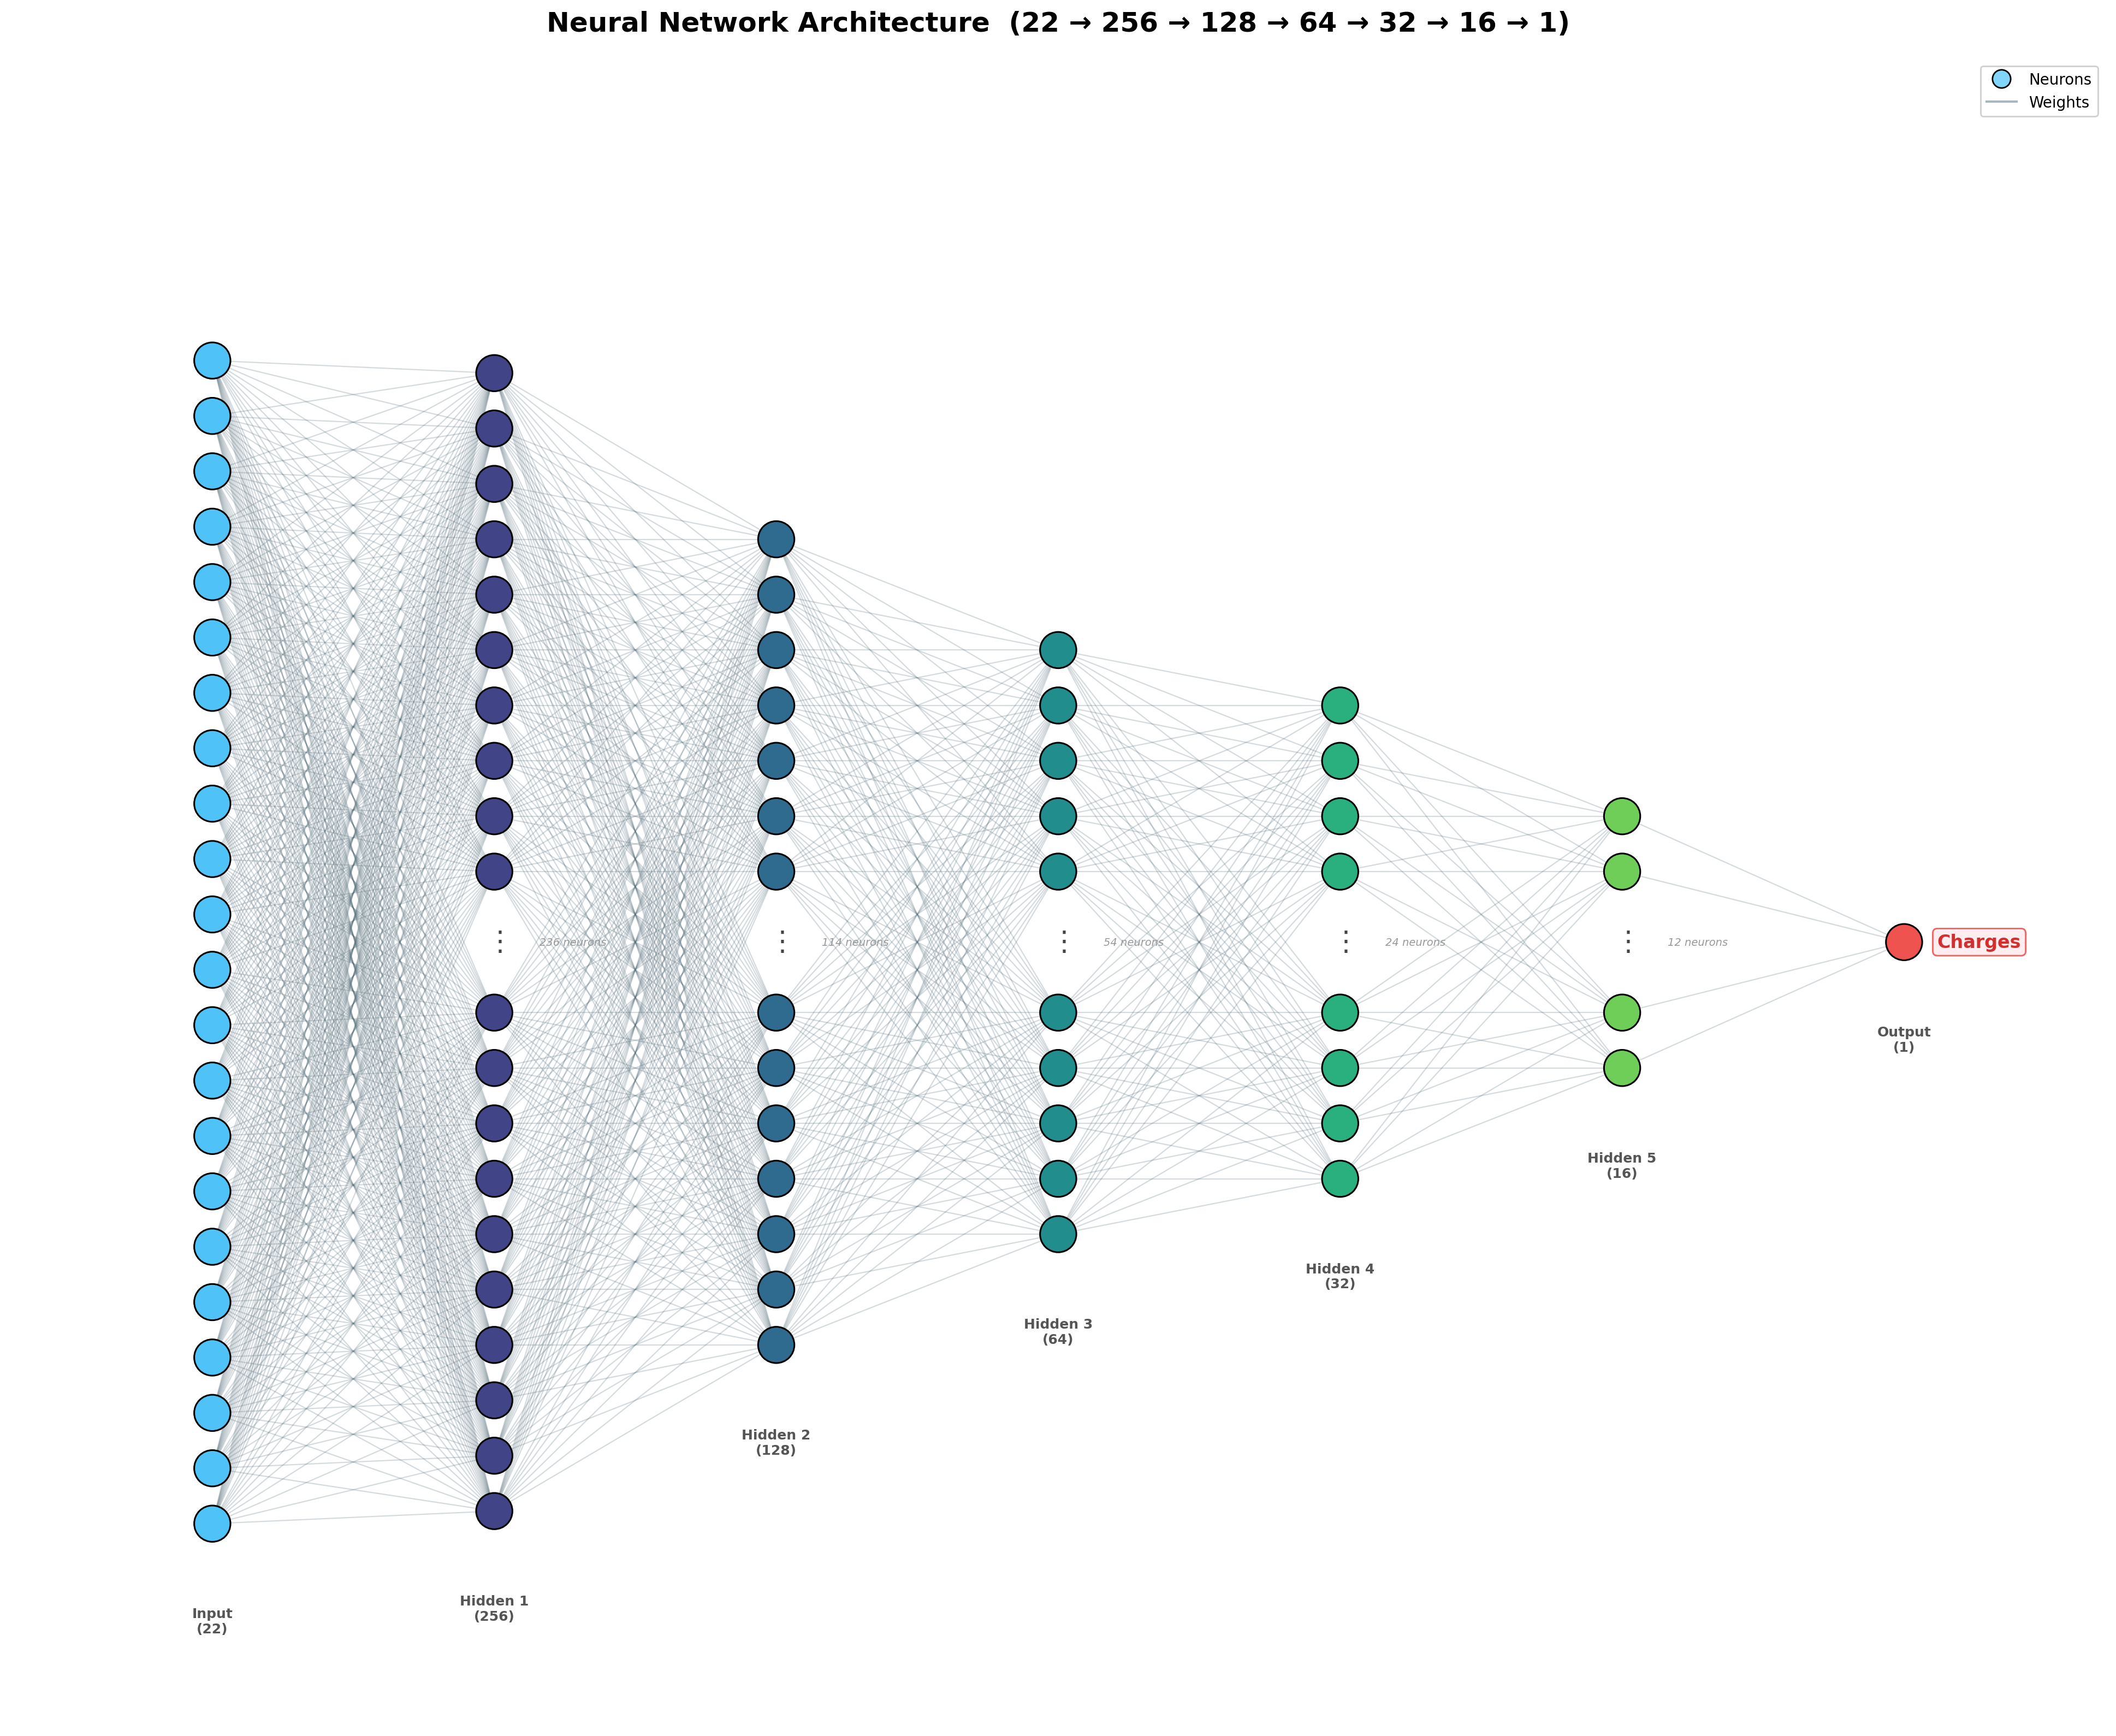
\includegraphics[width=0.85\textwidth]{Thesis/Chapter 2/Figures/nn_architecture (1).png}
    \caption{Candidate DNN architecture.}
    \label{fig:dnn_architecture}
\end{figure}

\noindent
The final output neuron represents the predicted health insurance charge or
premium. This architecture starts with a wide hidden layer and progressively
compresses the representation through successive layers, allowing the network to
learn nonlinear representations before reducing them to a scalar prediction.

\noindent
The architecture used in the empirical chapter may be implemented without
explicit bias vectors, depending on the final modelling choice confirmed for the
study. In that case, the layer recursion in
equations~\eqref{eq:pre_activation}-\eqref{eq:activation} simplifies to
\begin{equation}
\label{eq:bias_free_recursion}
    \mathbf{z}^{(l)}_i
    =
    \left(W^{(l)}\right)^{\top}
    \mathbf{a}^{(l-1)}_i,
    \qquad
    \mathbf{a}^{(l)}_i
    =
    \sigma_l
    \!\left(
        \mathbf{z}^{(l)}_i
    \right),
    \qquad
    l=1,\ldots,L,
\end{equation}
\equationlistentry{Layer recursion without bias}
with \(\mathbf{a}^{(0)}_i = \mathbf{x}_i\) as in
equation~\eqref{eq:input_layer}. The output prediction is then
\[
    f_{\theta}(\mathbf{x}_i)
    =
    a^{(L)}_{i1}.
\]
This bias-free specification removes additive layer-bias parameters from the
network architecture; the distinction between architectural, statistical and
data-related meanings of bias is noted above. Its adequacy is assessed empirically
through training, validation and test performance, and where appropriate through
comparison with a bias-inclusive network. One theoretical qualification should
be recorded. The approximation theorems reviewed in
Section~\ref{sec:dnn_regression} assume affine layer maps comprising both
weights and biases; a bias-free network whose activation satisfies
\(\sigma(0)=0\) is positively homogeneous and constrained to pass through the
origin of the standardised input space, so the universal approximation
guarantee does not directly apply to the implemented architecture.

\noindent
The final architecture should not be selected purely by intuition; it should be
determined using validation performance and evaluated on a held-out test set.
This is necessary because neural networks can be highly flexible. A network that
is too small may underfit, while a network that is too large may fit the
training data closely without generalising to unseen observations. The
DNN is therefore treated as a statistical learning model whose usefulness
is judged by out-of-sample prediction performance and by the quality of the
subsequent simulation and interpretability analysis
\citep{james2021introduction,hastie2009elements}.

\noindent
The dataset is partitioned as
\begin{equation}
\label{eq:data_partition}
    \mathcal{D}
    =
    \mathcal{D}_{\mathrm{train}}
    \cup
    \mathcal{D}_{\mathrm{val}}
    \cup
    \mathcal{D}_{\mathrm{test}},
\end{equation}
\equationlistentry{Training, validation and test partition}
where the three components are disjoint and exhaust \(\mathcal{D}\).  The
proportions allocated to each component are a design choice rather than a
fixed convention; the split used in this dissertation is stated in
Section~\ref{sec:feature_encoding_input_standardisation}. An epoch is one
complete pass through the training data. For a fitted parameter vector
\(\widehat{\theta}^{(e)}\) after epoch \(e\), the training and validation losses
are
\begin{equation}
\label{eq:training_loss_epoch}
    \mathcal{L}_{\mathrm{train}}^{(e)}
    =
    \frac{1}{n_{\mathrm{train}}}
    \sum_{i\in\mathcal{I}_{\mathrm{train}}}
    \left(
        y_i
        -
        f_{\widehat{\theta}^{(e)}}(\mathbf{x}_i)
    \right)^2
\end{equation}
\equationlistentry{Training loss at epoch $e$}
and
\begin{equation}
\label{eq:validation_loss_epoch}
    \mathcal{L}_{\mathrm{val}}^{(e)}
    =
    \frac{1}{n_{\mathrm{val}}}
    \sum_{i\in\mathcal{I}_{\mathrm{val}}}
    \left(
        y_i
        -
        f_{\widehat{\theta}^{(e)}}(\mathbf{x}_i)
    \right)^2.
\end{equation}
\equationlistentry{Validation loss at epoch $e$}
The candidate number of epochs is selected by comparing validation loss over the
epoch grid. If \(\mathcal{E}\) denotes the set of candidate epoch values, the
selected training duration is
\begin{equation}
\label{eq:epoch_selection}
    e^{\ast}
    =
    \arg\min_{e\in\mathcal{E}}
    \mathcal{L}_{\mathrm{val}}^{(e)}.
\end{equation}
\equationlistentry{Optimal epoch selection}
This validation step is necessary because training loss typically decreases as
the optimiser continues updating the model, but validation loss may eventually
increase if the network begins to adapt too closely to the training sample. A
decreasing training loss with a rising validation loss is a common indication of
overfitting, while weak training and validation performance may indicate
underfitting or unsuitable training settings.

\noindent
LOOCV is not adopted as the primary validation strategy. It would require
refitting the neural network once for each observation.

\noindent
Although \(K\)-fold cross-validation is often useful when a separate validation
set is unavailable or when dependence on a single random split must be reduced,
it is not required for the main analysis because the data are already supplied
with the fixed partition in equation~\eqref{eq:data_partition}. Applying
\(K\)-fold cross-validation to the full dataset would mix observations assigned
to validation and test components into the training process, weakening the
interpretation of the final test performance. Applying \(K\)-fold
cross-validation only to the training set would avoid this leakage, but would
require repeated DNN training across folds and candidate epoch values,
while the supplied validation set already provides the intended mechanism for
selecting the training duration. The validation analysis therefore uses the
pre-specified validation set to select \(e^{\ast}\), and the test set is used
only once for final model assessment.

% --------------------------------------------------------
% 2.4.3 Generalisation, Validation Analysis and
%       Bias-Variance Trade-off
% --------------------------------------------------------
\subsubsection{Generalisation, validation analysis and bias-variance trade-off}
\label{sec:generalisation_validation_bias_variance}

\noindent
The tension between overfitting and underfitting is particularly acute for
flexible models such as DNNs, which may contain many trainable
parameters and can represent complex nonlinear relationships. The formal
bias-variance decomposition below makes this trade-off precise.

\noindent
Expressing the regression formulation in equation~\eqref{eq:regression} in
population-level notation,
\begin{equation}
\label{eq:general_regression}
    Y
    =
    f(\mathbf{X})
    +
    \varepsilon,
\end{equation}
\equationlistentry{Population regression formulation}
where \(f(\mathbf{X})\) denotes the true regression function
\(m(\cdot)\) from equation~\eqref{eq:regression} and \(\varepsilon\) represents
irreducible noise with \(\mathbb{E}(\varepsilon\mid\mathbf{X})=0\). In the
homoscedastic case, the irreducible variation is denoted
\(\sigma_{\varepsilon}^{2}\).

\noindent
If \(\widehat{f}_{\mathcal{D}}\) is a model trained on a dataset
\(\mathcal{D}\), then prediction error on a new observation depends not only on
how well the model fits the observed data, but also on how stable the fitted
function is across different possible training samples. This motivates the
bias-variance trade-off in statistical learning
\citep{hastie2009elements,james2021introduction,bishop2006pattern}.

\noindent
For squared-error loss, the expected prediction error at a point
\(\mathbf{x}\) can be decomposed into three components:
\begin{equation}
\label{eq:bias_variance_pointwise}
\mathbb{E}_{\mathcal{D},Y}
\!\left[
\left(
Y - \widehat{f}_{\mathcal{D}}(\mathbf{x})
\right)^2
\right]
=
\underbrace{\left(
f(\mathbf{x})
-
\mathbb{E}_{\mathcal{D}}
\!\left[
\widehat{f}_{\mathcal{D}}(\mathbf{x})
\right]
\right)^2}_{\mathrm{Bias}^{2}}
+
\underbrace{
\mathbb{E}_{\mathcal{D}}
\!\left[
\left(
\widehat{f}_{\mathcal{D}}(\mathbf{x})
-
\mathbb{E}_{\mathcal{D}}
\!\left[
\widehat{f}_{\mathcal{D}}(\mathbf{x})
\right]
\right)^2
\right]
}_{\mathrm{Variance}}
+
\underbrace{\sigma_{\varepsilon}^{2}}_{\mathrm{Noise}}.
\end{equation}
\equationlistentry{Pointwise bias-variance decomposition}
The bias term measures the systematic error introduced by the choice of model
class, while the variance term measures the instability of the fitted model
across different training samples. The noise term
\(\sigma_{\varepsilon}^{2}\) represents irreducible variation in the response
that cannot be removed by any model based on the available predictors.

\noindent
The bias-variance trade-off can therefore be summarised as
\[
    \mathrm{Expected\ test\ error}
    =
    \mathrm{Variance}
    +
    \mathrm{Bias}^{2}
    +
    \mathrm{Irreducible\ noise}.
\]
Equivalently, in terms of model complexity,
\[
    \mathrm{Model\ complexity}\uparrow
    \quad
    \Longrightarrow
    \quad
    \mathrm{Bias}^{2}\downarrow,
    \qquad
    \mathrm{Variance}\uparrow,
\]
whereas
\[
    \mathrm{Model\ complexity}\downarrow
    \quad
    \Longrightarrow
    \quad
    \mathrm{Bias}^{2}\uparrow,
    \qquad
    \mathrm{Variance}\downarrow.
\]
This relationship explains why a highly flexible model may fit the training data
closely but perform poorly on unseen observations, while an overly simple model
may fail to capture the underlying pattern in both training and unseen data. The
aim is not to minimise training error alone, but to find a level of model
complexity that gives a favourable balance between bias and variance.

\begin{figure}[H]
    \centering
    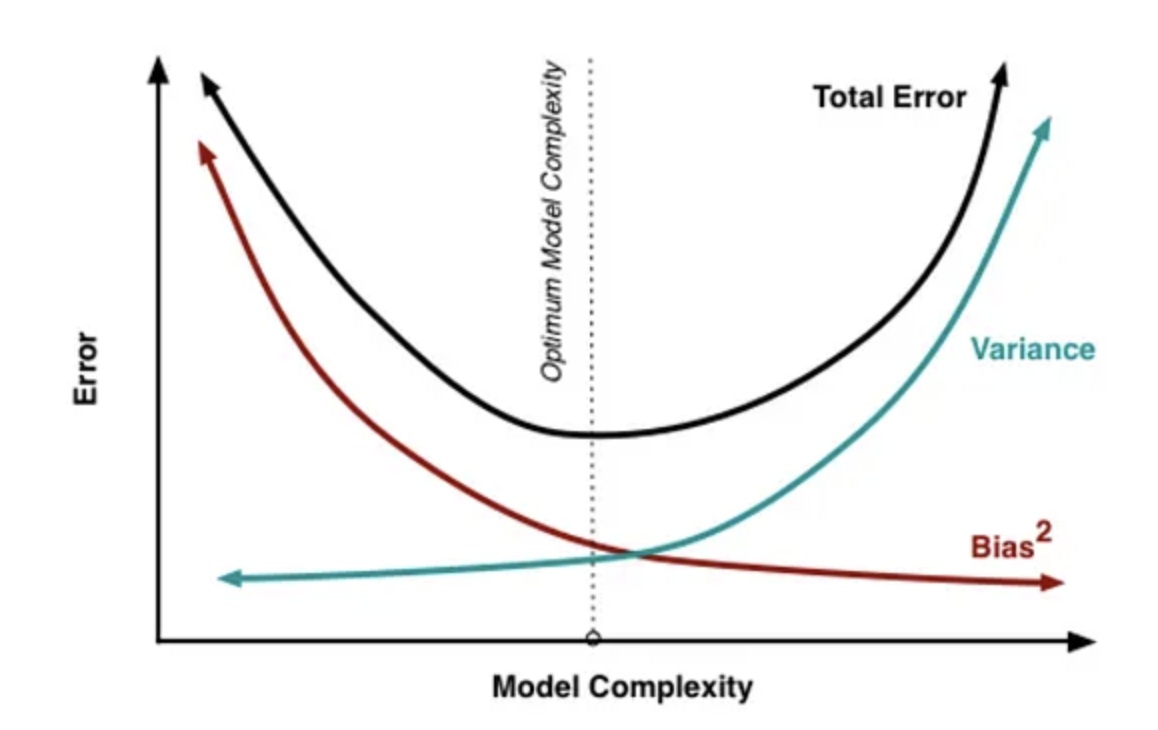
\includegraphics[width=0.72\textwidth]{Thesis/Chapter 2/Figures/bias_variance_tradeoff.png}
    \caption{Bias-variance trade-off illustration \citep{james2021introduction}.}
    \label{fig:bias_variance_tradeoff}
\end{figure}

\noindent
Figure~\ref{fig:bias_variance_tradeoff} provides a schematic illustration of
this relationship. The diagram emphasises that neither a very simple model nor
an excessively flexible model is generally desirable for prediction. Instead,
the preferred model complexity is the one that achieves the best out-of-sample
performance by balancing bias and variance. This principle motivates the
epoch-selection criterion defined in equation~\eqref{eq:epoch_selection}.

\noindent
The pointwise squared-error decomposition in
equation~\eqref{eq:bias_variance_pointwise} separates the expected prediction
error at a fixed input value \(\mathbf{x}\) into bias, variance and irreducible
noise. The same principle can also be expressed at the population level by
considering expected out-of-sample error. Let \(g^{(\mathcal{D})}\) denote a
fitted model obtained from a training sample \(\mathcal{D}\), and define the
average fitted model by
\[
    \bar{g}(\mathbf{x})
    =
    \mathbb{E}_{\mathcal{D}}
    \!\left[
        g^{(\mathcal{D})}(\mathbf{x})
    \right].
\]
Also let
\[
    m(\mathbf{X})
    =
    f(\mathbf{X})
    =
    \mathbb{E}(Y\mid \mathbf{X})
\]
denote the systematic component of the response, written with the
regression-function symbol \(m(\cdot)\) of equation~\eqref{eq:regression}
to avoid confusion with the bar notation used elsewhere for sample means. The expected out-of-sample
error under squared loss can then be written as
\begin{equation}
\label{eq:bias_variance_population}
\begin{aligned}
    \mathbb{E}_{\mathcal{D}}
    \!\left[
        E_{\mathrm{out}}
        \!\left(
            g^{(\mathcal{D})}
        \right)
    \right]
    &=
    \mathbb{E}_{\mathcal{D}}
    \!\left[
        \mathbb{E}_{\mathbf{X},Y}
        \!\left[
            \left(
                g^{(\mathcal{D})}(\mathbf{X}) - Y
            \right)^2
        \right]
    \right]
    \\[4pt]
    &=
    \underbrace{
    \mathbb{E}_{\mathbf{X}}
    \!\left[
        \mathbb{E}_{\mathcal{D}}
        \!\left[
            \left(
                g^{(\mathcal{D})}(\mathbf{X})
                -
                \bar{g}(\mathbf{X})
            \right)^2
        \right]
    \right]
    }_{\mathrm{Model\ variance}}
    \\[4pt]
    &\quad+
    \underbrace{
    \mathbb{E}_{\mathbf{X}}
    \!\left[
        \left(
            \bar{g}(\mathbf{X})
            -
            f(\mathbf{X})
        \right)^2
    \right]
    }_{\mathrm{Model\ bias}}
    +
    \underbrace{
    \mathbb{E}_{\mathbf{X}}
    \!\left[
        \mathbb{E}_{Y\mid\mathbf{X}}
        \!\left[
            \left(
                m(\mathbf{X})
                -
                Y
            \right)^2
        \right]
    \right]
    }_{\mathrm{Noise}}.
\end{aligned}
\end{equation}
\equationlistentry{Population expected prediction error}
This form is useful because it links model complexity directly to expected
out-of-sample performance, which is the quantity approximated by the validation
and test-set analysis. Complex models may reduce model bias by representing
richer patterns, but they may also increase model variance by becoming sensitive
to the particular training sample. Simpler models may have lower variance, but
they may miss important nonlinear structure. The practical aim is therefore to
choose a model that captures stable structure without merely recalling noise in
the training data.

\noindent
The training partition \(\mathcal{D}_{\mathrm{train}}\)
(equation~\eqref{eq:data_partition}) is used to estimate model parameters through
gradient-based optimisation. The validation partition
\(\mathcal{D}_{\mathrm{val}}\) guides the choice of training duration via
the epoch-selection criterion in equation~\eqref{eq:epoch_selection}. The test partition
\(\mathcal{D}_{\mathrm{test}}\) is reserved for final out-of-sample evaluation
after the model has been selected and its architecture fixed. Using the test set
for any model-selection decision invalidates its role as an honest estimate of
generalisation performance
\citep{hastie2009elements,abu2012learning}.

\noindent
Generalisation is assessed by comparing training, validation and test
performance using RMSE, MAE and \ensuremath{R^2}. If
training performance is substantially better than validation or test
performance, this may indicate overfitting. If all three are weak, this may
indicate underfitting. If training, validation and test results are similar and
sufficiently strong, this supports the conclusion that the fitted model
generalises reasonably well within the available dataset.

\noindent
The use of a benchmark health insurance dataset introduces an additional
qualification: internal predictive validity within the dataset's
distributional domain must be distinguished from external validity for
real insurance populations with different risk profiles, benefit
structures or demographics.  The scope delimitations of
Section~\ref{sec:scope_delimitations} formalise this boundary.

\newpage
% =============================================================
% 2.5  Health Insurance Pricing and Cost Prediction
% =============================================================

\subsection{Health Insurance Pricing and Cost Prediction}
\label{sec:health_insurance_pricing_cost_prediction}

\noindent
The supervised-regression formulation gives the
statistical form of the empirical problem: the observed response \(y_i\) is a
continuous monetary outcome, and the fitted function
\(\widehat{m}(\mathbf{x})\) maps policyholder attributes to a predicted cost.
The health insurance setting gives this regression problem its actuarial
meaning. A predicted monetary outcome is not merely an abstract response
variable; it is connected to premium rating, claim-cost estimation and risk
segmentation. Classical actuarial pricing often relies on transparent
regression-based models, especially GLMs, while the
DNN considered here plays the related role of a flexible nonlinear
estimator of the cost surface rather than a replacement for actuarial reasoning.

\noindent
The broader actuarial machine-learning literature provides extensive evidence
that neural networks and related models can be embedded within traditional
insurance frameworks.  \citet{wuthrich2023statistical} provide a comprehensive
treatment of statistical foundations for actuarial learning,
\citet{noll2020case} demonstrate neural-network pricing on French motor
third-party liability data, and \citet{schelldorfer2019nesting} show how
classical actuarial models can be nested within neural-network architectures.
\citet{blierwong2021machine} survey machine-learning applications across
property and casualty insurance pricing and reserving.  In the life insurance
domain, \citet{blomerus2025longterm} demonstrates the viability of deep
learning for long-term life insurance valuations using commercial European
portfolio data, achieving valuations sufficiently accurate to support
capital calculations under Solvency~II; the 99.5\% figure in that
framework is the confidence level of the one-year Value-at-Risk defining
the Solvency Capital Requirement, rather than a prescribed valuation
accuracy standard.

\noindent
Within health insurance specifically, recent work has demonstrated that neural
networks can be incorporated into actuarial pricing structures without
abandoning the underlying frequency-severity logic.
\citet{laporta2025neural} propose neural-network models for pricing correlated
health risks by embedding negative multinomial
neural networks for claim frequency and gamma neural networks for claim
severity within a classical frequency-severity structure. Their empirical
results on real-world health insurance data show that neural-network models
achieve lower out-of-sample deviance and better risk diversification than
established regression methods such as GLMs, as measured
by the ABC lift metric. The relevance of this work is that neural networks need
not be treated as generic black-box alternatives; they can be incorporated
within actuarial pricing logic to improve both accuracy and risk segmentation.

\noindent
A complementary approach to neural-network pricing is to impose explicit shape
constraints during training.  \citet{richman2024icenet} develop the ICEnet,
which adds smoothness and monotonicity penalty terms to the loss function so
that the network's ICE outputs vary in a manner
consistent with actuarial domain knowledge.  Applied to claims frequency
prediction on the French motor third-party liability dataset, the ICEnet
achieves a test-set Poisson deviance within $0.0001$ of the unconstrained
network, demonstrating that actuarial reasonableness can be enforced with
negligible accuracy cost.  Because the ICEnet targets count data under a
Poisson deviance criterion, its results are not directly comparable with the
continuous monetary cost predictions in the present dissertation; a
methodological comparison is presented in
Section~\ref{sec:comparison_constrained_nn}.

\noindent
Alongside neural-network approaches, tree-based ensemble methods have become
widely used for insurance cost prediction on structured tabular data.
\citet{orji2024explainable} apply RFs and gradient-boosted trees to
health insurance cost data and report predictive performance comparable to, and
in some configurations exceeding, that of neural networks.  More broadly,
\citet{grinsztajn2022why} provide systematic evidence that tree-based models,
particularly gradient-boosted implementations such as XGBoost
\citep{chen2016xgboost}, building on the gradient boosting framework of
\citet{friedman2001greedy}, frequently match or outperform DNNs
on
medium-sized tabular datasets of the kind encountered in actuarial practice.
Because insurance cost prediction is fundamentally an actuarial problem defined
on structured policyholder attributes rather than on unstructured data such as
images or text, tree-based methods represent a credible alternative to the
DNN and may in some settings be the preferred model class.  The present
dissertation nonetheless selects the DNN as the primary model for the
MC and Shapley workflow because it provides a differentiable
prediction surface compatible with gradient-based SHAP explainers and
with continuous forward-pass evaluation over large simulated input samples;
the specific gradient-based explainer employed is described in
Chapter~\ref{chap:methods_and_data}.  An RF
and an XGBoost regressor are fitted as benchmarks to contextualise the
DNN's predictive performance within this spectrum of model classes.

\noindent
Earlier work on algorithmic health cost prediction by
\citet{bertsimas2008algorithmic} demonstrated the potential of machine-learning
methods to outperform traditional actuarial approaches, while
\citet{duncan2016testing} tested alternative regression frameworks for
predictive modelling of healthcare costs in the North American context.
These studies confirm that health insurance cost prediction is a well-studied
regression problem where model flexibility can yield meaningful improvements
over simpler specifications.

\noindent
The available Kaggle insurance data \citep{kaggleInsuranceDataML} do not provide separate claim-frequency and
claim-severity processes. A separate actuarial claims model is therefore not
fitted. Instead, the observed monetary response is treated as an aggregate
health insurance charge or premium proxy, and cost prediction is formulated as a
supervised regression problem. This gives a narrower empirical objective: to
study how a fitted nonlinear prediction surface behaves on a benchmark
health insurance dataset, without claiming to reproduce the complete pricing
tariff or underwriting rules of a specific insurer.

\noindent
The objective is not merely to obtain a point estimate of cost for each
policyholder, but to understand the distribution and drivers of predicted costs
under varying input profiles. This is important because actuarial modelling is
concerned not only with average prediction, but also with uncertainty,
high-cost scenarios and the interpretation of risk drivers
\citep{denuit2007actuarial}. In this sense, the fitted regression function
\(\widehat{m}\) is the starting point for a broader analysis of predicted-cost
behaviour rather than the end of the modelling exercise.

\noindent
Health expense projection literature provides a further actuarial motivation for studying predicted costs distributionally. \citet{christiansen2018projection}
develop practical models for projecting health insurance expenditures over
short time horizons, which supports the view that health cost analysis should
consider the behaviour of cost outcomes beyond isolated point estimates. The
present dissertation differs from traditional health expense projection because
it does not construct a demographic, utilisation or claims-process model.
Instead, it trains a DNN on policyholder-level attributes and uses Monte
Carlo input simulation to examine the distribution of costs implied by the
fitted prediction function. This distinction keeps the empirical claim modest:
the analysis concerns model-implied predicted costs under the selected
benchmark-data and simulation design, rather than realised expenditure
dynamics in an insurer's full portfolio.

\noindent
Ordinary cost prediction is therefore extended in two ways. First, after fitting
the DNN, MC input simulation is used to generate many
possible policyholder profiles and examine the distribution of model-implied
predicted costs. Second, Shapley-value interpretation is used to identify the
variables that drive individual predictions and high-cost simulated profiles.
This connects health insurance cost prediction with simulation-based risk
analysis and explainable machine learning. The resulting analysis asks not only
how accurately the fitted model predicts costs, but also how predicted costs
vary across simulated profiles and which variables the model attributes to the
upper tail of the predicted-cost distribution.

\noindent
The interpretation remains model-based: the MC distribution describes
variation in fitted predictions under the selected input distribution, and
Shapley values explain the fitted DNN's predictions relative to the
chosen background distribution.  The causal and scope delimitations stated in
Section~\ref{sec:scope_delimitations} apply throughout.  The health insurance
application is therefore used as an actuarially motivated setting in which
prediction, simulation and explanation can be combined while keeping the
empirical claims within the limits of the data.


\newpage

% =============================================================
% 2.6  Input Distribution Diagnostics for Simulation
% =============================================================

\subsection{Input Distribution Diagnostics for Simulation}
\label{sec:input_distribution_diagnostics}

\noindent
The validation analysis of
Section~\ref{sec:generalisation_validation_bias_variance} addresses whether
the fitted DNN generalises within the supplied
training, validation and test structure, but MC input simulation requires an
additional diagnostic step. Even when a fitted prediction function
\(f_{\widehat{\theta}}\) has acceptable validation and test performance, the
simulation results may be misleading if the input profiles are generated from an
unrealistic or poorly specified input distribution. The diagnostic concern
therefore shifts from the fitted model itself to the probability law used to
generate simulated policyholder profiles.

\noindent
A trained model \(f_{\widehat{\theta}}\) can be evaluated at any admissible
input vector, but simulation-based analysis requires a probability law for the
random input vector \(\mathbf{X}\). The distribution of simulated predictions
depends not only on the fitted DNN, but also on the assumed or estimated
distribution of policyholder attributes. Input distribution diagnostics therefore
provide the empirical basis for specifying the input distribution
\(\widehat{F}_{X}\) used later in the MC component of the framework.

\noindent
Let
\[
    \mathbf{X}
    =
    (X_1,\ldots,X_p)^{\top}
\]
denote the vector of input variables before final model encoding, and let
\(\widetilde{\mathbf{X}}\) denote the corresponding model-ready vector after
encoding and standardisation. Where no ambiguity arises, \(\mathbf{X}\) is used
as the generic random input vector. Before specifying an input distribution for
\(\mathbf{X}\), the empirical distribution of each variable must be examined.
For numerical variables, this includes measures of location, scale, skewness,
tail behaviour and possible outliers. For categorical variables, this includes
category frequencies, rare levels and possible class imbalance.

\noindent
For a numerical variable \(X_j\), the sample mean and variance are
\[
    \bar{x}_j
    =
    \frac{1}{n}
    \sum_{i=1}^{n}
    x_{ij},
    \qquad
    s_j^2
    =
    \frac{1}{n-1}
    \sum_{i=1}^{n}
    \left(
        x_{ij} - \bar{x}_j
    \right)^2.
\]
Skewness can be estimated by
\[
    \widehat{\gamma}_{1j}
    =
    \frac{
    \frac{1}{n}\sum_{i=1}^{n}
    \left(
        x_{ij}-\bar{x}_j
    \right)^3
    }{
    \left[
    \frac{1}{n}\sum_{i=1}^{n}
    \left(
        x_{ij}-\bar{x}_j
    \right)^2
    \right]^{3/2}
    },
\]
and kurtosis by
\[
    \widehat{\gamma}_{2j}
    =
    \frac{
    \frac{1}{n}\sum_{i=1}^{n}
    \left(
        x_{ij}-\bar{x}_j
    \right)^4
    }{
    \left[
    \frac{1}{n}\sum_{i=1}^{n}
    \left(
        x_{ij}-\bar{x}_j
    \right)^2
    \right]^2
    }.
\]
Following common convention, the sample variance \(s_j^2\) uses the
unbiased divisor \(n-1\), whereas the skewness and kurtosis estimators are
ratios of divisor-\(n\) central moments; this mixed convention is adopted
throughout. Values of \(\widehat{\gamma}_{1j}>0\) indicate right-skewness, while values of
\(\widehat{\gamma}_{2j}\) substantially above \(3\) indicate heavier-than-normal
tails. These quantities help identify variables that are asymmetric,
heavy-tailed or potentially unsuitable for simple symmetric distributional
assumptions.

\noindent
The response variable \texttt{charges} is also subject to diagnostic analysis,
even though MC input simulation focuses primarily on the predictors.
Insurance cost variables often display right-skewness, heterogeneity and
upper-tail behaviour \citep{denuit2007actuarial}. If the response is strongly
skewed, a log transformation of the form
\[
    Y_i^{*}
    =
    \log(1+Y_i)
\]
may be considered during model training. If such a transformation is used, final
predictions and performance metrics must be back-transformed and reported on the
original monetary scale.

\noindent
For categorical variables, the relevant diagnostic is the empirical frequency
distribution. If \(X_j\) takes values in the finite set
\(\{c_1,\ldots,c_{K_j}\}\), the empirical proportion of category \(c_k\) is
\[
    \widehat{p}_{jk}
    =
    \frac{1}{n}
    \sum_{i=1}^{n}
    \mathbb{I}\{X_{ij}=c_k\}.
\]
Rare categories may be poorly represented in the training set and may lead to
unstable predictions or unreliable Shapley summaries. In the health insurance
setting, categorical variables such as region, smoking status, medical history,
exercise frequency, occupation and coverage level may all influence the
structure learned by the fitted model.

\noindent
Input diagnostics also inform preprocessing. Numerical variables are
standardised before training a DNN to support numerical stability in
gradient-based optimisation. The standardisation parameters must be computed from
the training set only and then applied to the validation and test sets using
those same training-set values, so that information from held-out observations
does not leak into the training procedure. The specific standardisation formula
and its implementation are detailed in Chapter~\ref{chap:methods_and_data}.

\noindent
Validation analysis assesses whether
\(f_{\widehat{\theta}}\) performs adequately on held-out observations from the
available data distribution. Input distribution diagnostics assess whether the
profiles generated for MC simulation remain compatible with that same
empirical domain. Without both checks, the subsequent predicted-cost
distribution and high-cost Shapley summaries could reflect unrealistic simulated
profiles rather than meaningful behaviour of the fitted model.

% =============================================================
% 2.7  Specification of the Input Distribution
% =============================================================

\subsection{Specification of the Input Distribution}
\label{sec:input_simulation_uncertainty_dependence}

\noindent
The input distribution
\(\widehat{F}_{X}\) was defined as a product of independent fitted marginals
(equation~\eqref{eq:input_law}), with the sampling and propagation
procedure given by equations~\eqref{eq:mc_sample_framework}
and~\eqref{eq:mc_predictions_framework}. Three main
approaches are available for constructing \(\widehat{F}_{X}\).

\noindent
The simplest approach is empirical row resampling, in which complete observed
covariate vectors are sampled from the dataset with replacement
\citep{efron1993bootstrap}:
\begin{equation}
\label{eq:row_resampling}
    \mathbf{X}^{(\ell)}
    \in
    \{\mathbf{x}_1,\ldots,\mathbf{x}_n\},
    \qquad
    \ell=1,\ldots,M.
\end{equation}
\equationlistentry{Empirical row resampling}
Because the full covariate vector is sampled as a unit, empirical row resampling
retains whatever joint structure is present in the observed data. Its limitation
is that it cannot generate policyholder profiles outside the observed data
range.

\noindent
A second approach is marginal parametric simulation, in which each input
variable is assigned a fitted marginal distribution
\citep{rubinstein2016simulation,glasserman2004monte}. For a numerical variable
\(X_j\), a parametric family \(F_j(\,\cdot\,;\psi_j)\) may be fitted by maximum
likelihood:
\begin{equation}
\label{eq:mle_marginal}
    \widehat{\psi}_j
    =
    \arg\max_{\psi_j}
    \sum_{i=1}^{n}
    \log f_j(x_{ij};\psi_j),
\end{equation}
\equationlistentry{Maximum likelihood for marginal parameters}
where \(f_j(\cdot;\psi_j)\) is the corresponding density or probability mass
function. Simulated values are then drawn as
\begin{equation}
\label{eq:marginal_draw}
    X_j^{(\ell)}
    \sim
    F_j(\,\cdot\,;\widehat{\psi}_j),
    \qquad
    \ell=1,\ldots,M.
\end{equation}
\equationlistentry{Draw from fitted marginal distribution}
This approach is convenient and can generate values beyond the observed sample.
It is the approach adopted in this dissertation, where independent fitted
marginals are combined as specified in equation~\eqref{eq:input_law}. The
independence assumption is a deliberate modelling choice, as discussed in
connection with equation~\eqref{eq:input_law}. Two strands of literature
qualify this choice. Evaluating or explaining a fitted model at covariate
combinations that lie off the data manifold can produce extrapolation
artefacts, because the model is queried in regions where it was never
constrained by training data \citep{hooker2021unrestricted}. Relatedly, when
features are dependent, the marginal (interventional) and conditional
formulations of Shapley attribution diverge, and estimating the conditional
expectations required by the latter is non-trivial
\citep{aas2021explaining, janzing2020feature}. Under the product-marginal
design adopted here the two formulations coincide by construction, which is
precisely the condition under which the marginal SHAP estimator used
later is internally consistent. The generated profiles may nonetheless
include jointly implausible attribute combinations, so attribution results
in sparsely supported regions of the input space must be interpreted with
care.

\noindent
A third approach is nonparametric or semi-parametric simulation, using
bootstrap-type resampling or smoothed empirical distributions
\citep{efron1993bootstrap}. These methods avoid imposing a strong parametric
form on the marginal distributions, although they remain limited by the
information contained in the observed sample. Their usefulness depends on
whether the empirical data provide sufficient coverage of the regions of the
input space that are relevant for the simulation exercise.

\noindent
The choice of specification method determines the input profiles passed through
the fitted prediction function. A poorly specified input distribution may create
high-cost profiles that are artefacts of the simulation design rather than
meaningful evaluations of the fitted model.

\noindent
Figure~\ref{fig:input_law_construction} illustrates the marginal parametric
construction adopted here. Each column of \(\mathcal{X}_{\mathrm{train}}\) is
fitted independently to a parametric marginal distribution, and the product of
these marginals defines \(\widehat{F}_{X}\), from which \(M\) synthetic input
vectors are drawn to form the simulation design matrix.

\begin{figure}[H]
\centering
\begin{tikzpicture}[
    databox/.style={rectangle, draw, minimum width=2cm,
        minimum height=0.9cm, align=center, font=\small},
    prodbox/.style={rectangle, draw, rounded corners,
        minimum width=11.5cm, minimum height=1.1cm,
        align=center, font=\normalsize, fill=blue!8},
    samplebox/.style={rectangle, draw, rounded corners,
        fill=purple!5, inner sep=10pt,
        align=center, font=\small},
    arr/.style={->, thick, >=stealth}
]

\def\colA{0}
\def\colB{3}
\def\colMid{5}
\def\colC{7}
\def\colD{10}

% ROW 1 — Training attribute columns
\node[databox] (x1) at (\colA,0)
      {$\mathbf{x}_{\cdot 1}$\\{\scriptsize(age)}};
\node[databox] (x2) at (\colB,0)
      {$\mathbf{x}_{\cdot 2}$\\{\scriptsize(BMI)}};
\node[font=\large] at (\colMid,0) {$\cdots$};
\node[databox] (x3) at (\colC,0)
      {$\mathbf{x}_{\cdot(p{-}1)}$\\{\scriptsize(children)}};
\node[databox] (xp) at (\colD,0)
      {$\mathbf{x}_{\cdot p}$\\{\scriptsize(smoker)}};

\node[font=\small\bfseries] at (\colMid,1.1)
      {Training attributes $\mathcal{X}_{\mathrm{train}}$};

% ROW 2 — Fitted-marginal labels
\node[font=\small, align=center] (f1) at (\colA,-1.9)
      {$\widehat{F}_{X_1}$\\[-1pt]{\scriptsize Normal}};
\node[font=\small, align=center] (f2) at (\colB,-1.9)
      {$\widehat{F}_{X_2}$\\[-1pt]{\scriptsize Lognormal}};
\node[font=\large] at (\colMid,-1.9) {$\cdots$};
\node[font=\small, align=center] (f3) at (\colC,-1.9)
      {$\widehat{F}_{X_{p-1}}$\\[-1pt]{\scriptsize Poisson}};
\node[font=\small, align=center] (fp) at (\colD,-1.9)
      {$\widehat{F}_{X_p}$\\[-1pt]{\scriptsize Categorical}};

\draw[arr] (x1) -- node[right,font=\scriptsize]{fit} (f1);
\draw[arr] (x2) -- node[right,font=\scriptsize]{fit} (f2);
\draw[arr] (x3) -- node[right,font=\scriptsize]{fit} (f3);
\draw[arr] (xp) -- node[right,font=\scriptsize]{fit} (fp);

% ROW 3 — Mini distribution plots
\begin{scope}[shift={(\colA,-3.15)}]
    \draw[gray!50] (-1,0) -- (1,0);
    \fill[blue!12]
        plot[smooth,domain=-0.9:0.9,samples=30]
        (\x,{0.6*exp(-5*\x*\x)})
        -- (0.9,0) -- (-0.9,0) -- cycle;
    \draw[thick,blue!70]
        plot[smooth,domain=-0.9:0.9,samples=30]
        (\x,{0.6*exp(-5*\x*\x)});
\end{scope}

\begin{scope}[shift={(\colB,-3.15)}]
    \draw[gray!50] (-1,0) -- (1.1,0);
    \fill[red!10]
        plot[smooth,domain=-0.7:1.05,samples=30]
        (\x,{0.55*exp(-3*(\x+0.1)*(\x+0.1))
             +0.15*exp(-5*(\x-0.6)*(\x-0.6))})
        -- (1.05,0) -- (-0.7,0) -- cycle;
    \draw[thick,red!70]
        plot[smooth,domain=-0.7:1.05,samples=30]
        (\x,{0.55*exp(-3*(\x+0.1)*(\x+0.1))
             +0.15*exp(-5*(\x-0.6)*(\x-0.6))});
\end{scope}

\node[font=\large] at (\colMid,-2.95) {$\cdots$};

\begin{scope}[shift={(\colC,-3.15)}]
    \draw[gray!50] (-1,0) -- (1.15,0);
    \foreach \lx/\rx/\ht in
        {-0.7/-0.4/0.35, -0.15/0.15/0.55,
         0.4/0.7/0.25,   0.85/1.05/0.08}{
        \fill[green!40] (\lx,0) rectangle (\rx,\ht);
        \draw[green!60!black] (\lx,0) rectangle (\rx,\ht);
    }
    \foreach \xv/\lab in {-0.55/0, 0/1, 0.55/2, 0.95/3}
        \node[font=\tiny] at (\xv,-0.15) {\lab};
\end{scope}

\begin{scope}[shift={(\colD,-3.15)}]
    \draw[gray!50] (-0.85,0) -- (0.85,0);
    \fill[yellow!50]   (-0.65,0) rectangle (-0.1,0.55);
    \draw[yellow!60!black] (-0.65,0) rectangle (-0.1,0.55);
    \fill[yellow!50]   (0.1,0) rectangle (0.65,0.2);
    \draw[yellow!60!black] (0.1,0) rectangle (0.65,0.2);
    \node[font=\tiny] at (-0.375,-0.15) {No};
    \node[font=\tiny] at ( 0.375,-0.15) {Yes};
\end{scope}

% ROW 4 — Product of independent marginals
\node[prodbox] (FX) at (\colMid,-4.85)
      {$\displaystyle\widehat{F}_{X}
        \;=\;\prod_{j=1}^{p}\widehat{F}_{X_j}$};

\draw[arr] (\colA,-3.55) -- (FX.north -| \colA,0);
\draw[arr] (\colB,-3.55) -- (FX.north -| \colB,0);
\draw[arr] (\colC,-3.55) -- (FX.north -| \colC,0);
\draw[arr] (\colD,-3.55) -- (FX.north -| \colD,0);

\node[below=0.2cm of FX, font=\scriptsize\itshape] (indep)
      {(independent marginals; no copula structure)};

% ROW 5 — Sampled design matrix
\draw[arr] (indep.south) ++(0,-0.15) -- ++(0,-0.8)
      node[midway,right,font=\scriptsize]{sample $M$ vectors};

\node[samplebox] at (\colMid,-8.6)
      {$\underbrace{%
       \begin{pmatrix}
       x_1^{(1)} & x_2^{(1)} & \cdots & x_p^{(1)}\\[3pt]
       x_1^{(2)} & x_2^{(2)} & \cdots & x_p^{(2)}\\[1pt]
       \vdots    & \vdots    & \ddots & \vdots   \\[1pt]
       x_1^{(M)} & x_2^{(M)} & \cdots & x_p^{(M)}
       \end{pmatrix}
       }_{\displaystyle
         \mathcal{X}_{\mathrm{sim}}\;\in\;\mathbb{R}^{M\times p}}$};

\end{tikzpicture}
\caption{Construction of the input distribution $\widehat{F}_{X}$.}
\label{fig:input_law_construction}
\end{figure}

% =============================================================
% 2.8  Foundations of MC
% =============================================================

\subsection{Foundations of MC}
\label{sec:monte_carlo_foundations}

\noindent
MC simulation rests on a small number of foundational results
concerning the crude MC estimator, its convergence
properties and the precision measures that underpin the analysis
\citep{glasserman2004monte, rubinstein2016simulation, robert2004monte,
kroese2011handbook}.

\noindent
Let \(X\) be a random variable with distribution \(F\), and suppose that the
quantity of interest is
\begin{equation}
\label{eq:mc_target}
    \theta
    =
    \mathbb{E}[g(X)].
\end{equation}
\equationlistentry{Target quantity as expectation}
If
\begin{equation}
\label{eq:mc_iid_sample}
    X^{(1)},\ldots,X^{(M)}
    \stackrel{\mathrm{iid}}{\sim}
    F,
\end{equation}
\equationlistentry{IID sample from distribution $F$}
then the crude MC estimator of \(\theta\) is
\begin{equation}
\label{eq:mc_estimator}
    \widehat{\theta}_{M}
    =
    \frac{1}{M}
    \sum_{\ell=1}^{M}
    g
    \!\left(
        X^{(\ell)}
    \right).
\end{equation}
\equationlistentry{Crude MC estimator}
Under standard regularity conditions, the law of large numbers implies
\begin{equation}
\label{eq:mc_lln}
    \widehat{\theta}_{M}
    \longrightarrow
    \theta
    \qquad
    \text{as}
    \qquad
    M\longrightarrow\infty.
\end{equation}
\equationlistentry{Law of large numbers for MC}
If
\begin{equation}
\label{eq:mc_variance_condition}
    \sigma_g^2
    =
    \mathrm{Var}\{g(X)\}
    <
    \infty,
\end{equation}
\equationlistentry{Variance condition for $g(X)$}
then
\begin{equation}
\label{eq:mc_estimator_variance}
    \mathrm{Var}
    \!\left(
        \widehat{\theta}_{M}
    \right)
    =
    \frac{\sigma_g^2}{M},
\end{equation}
\equationlistentry{Variance of MC estimator}
which yields the familiar \(M^{-1/2}\) convergence rate of ordinary MC
simulation \citep{caflisch1998monte,glasserman2004monte}.

\noindent
The MCSE quantifies the simulation error associated with
using a finite number of random draws. It is estimated by
\begin{equation}
\label{eq:mcse}
    \mathrm{MCSE}
    \!\left(
        \widehat{\theta}_{M}
    \right)
    =
    \frac{s_M}{\sqrt{M}},
\end{equation}
\equationlistentry{MCSE}
where
\begin{equation}
\label{eq:mc_sample_variance}
    s_M^2
    =
    \frac{1}{M-1}
    \sum_{\ell=1}^{M}
    \left[
        g
        \!\left(
            X^{(\ell)}
        \right)
        -
        \widehat{\theta}_{M}
    \right]^2.
\end{equation}
\equationlistentry{Sample variance for MCSE}
By the central limit theorem,
\begin{equation}
\label{eq:mc_clt}
    \frac{
        \widehat{\theta}_{M}
        -
        \theta
    }{
        s_M/\sqrt{M}
    }
    \;
    \overset{d}{\longrightarrow}
    \;
    N(0,1),
\end{equation}
\equationlistentry{Central limit theorem for MC}
giving the approximate \(100(1-\alpha)\%\) MC confidence interval
\begin{equation}
\label{eq:mc_ci}
    \widehat{\theta}_{M}
    \pm
    z_{1-\alpha/2}
    \frac{s_M}{\sqrt{M}}.
\end{equation}
\equationlistentry{MC confidence interval}
This interval describes uncertainty due to the finite number of MC
draws. It does not, by itself, represent all sources of statistical uncertainty
in the fitted DNN, the input distribution or the realised insurance cost.

\noindent
In the health insurance framework, the function \(g\) is
the fitted prediction function \(\widehat{m}\), the distribution \(F\) is the
fitted input distribution \(\widehat{F}_{X}\), and the target
\(\theta\) corresponds to summaries of the model-implied predicted-cost
distribution such as the mean, variance and upper-tail probabilities. The
convergence, variance and confidence-interval results above therefore apply
directly to those summaries.

% =============================================================
% 2.9  Variance Reduction and Tail Simulation
% =============================================================

\subsection{Variance Reduction and Tail Simulation}
\label{sec:variance_reduction_tail_simulation}

\noindent
For many quantities, ordinary MC simulation is sufficient when the
simulation budget is large and the MCSE is reported.
However, when the quantity of interest is a tail probability, a high quantile or
a rare high-cost event, crude MC can become inefficient because few
simulated draws fall in the region of interest. This issue is directly relevant
to insurance because high-cost events may be financially important even when
they are relatively rare \citep{glasserman2004monte}.  The statistical
modelling of extreme events is well developed in the quantitative risk
management literature \citep{mcneil2015quantitative, embrechts1997modelling,
coles2001introduction}, where tail behaviour is characterised through extreme
value distributions and related threshold exceedance models.

\noindent
Two clarifications situate the present tail analysis within this
literature. First, the quantity simulated here is the fitted conditional
mean \(\widehat{m}(\mathbf{X})\), so the upper tail examined is a tail of
conditional means rather than of realised costs; since
\(\mathrm{Var}\{\mathbb{E}(Y\mid\mathbf{X})\}\leq\mathrm{Var}(Y)\), this
tail is necessarily lighter than the tail of realised claim costs, and
high-cost conditioning statements therefore concern expected costs rather
than realised claim severities. Second, a fuller treatment of extremes
would adopt the peaks-over-threshold framework, in which suitably
normalised excesses over a high threshold converge to the generalised
Pareto distribution
\citep{pickands1975statistical, balkema1974residual, coles2001introduction};
fitting such threshold-exceedance models to the cost distribution is
deferred to future work.

\noindent
Let \(u\) denote a high-cost threshold, and suppose that the model-implied
exceedance probability is
\[
    p_u
    =
    \mathbb{P}
    \!\left(
        \widehat{Y}>u
    \right),
\]
where
\[
    \widehat{Y}
    =
    \widehat{m}(\mathbf{X}),
    \qquad
    \mathbf{X}
    \sim
    \widehat{F}_{X}.
\]
Given simulated predictions
\(\widehat{Y}^{(1)},\ldots,\widehat{Y}^{(M)}\), the crude MC estimator
of \(p_u\) is
\[
    \widehat{p}_u
    =
    \frac{1}{M}
    \sum_{\ell=1}^{M}
    \mathbb{I}
    \!\left\{
        \widehat{Y}^{(\ell)}>u
    \right\}.
\]
Its estimated standard error is
\[
    \widehat{\mathrm{SE}}
    \!\left(
        \widehat{p}_u
    \right)
    =
    \sqrt{
        \frac{
            \widehat{p}_u
            \left(
                1-\widehat{p}_u
            \right)
        }{
            M
        }
    }.
\]
The relative standard error is approximately
\[
    \frac{
        \widehat{\mathrm{SE}}
        \!\left(
            \widehat{p}_u
        \right)
    }{
        \widehat{p}_u
    }
    \approx
    \sqrt{
        \frac{
            1-\widehat{p}_u
        }{
            M\widehat{p}_u
        }
    }.
\]
When \(p_u\) is small, the expected number of exceedances,
\(Mp_u\), may remain small unless \(M\) is large. This explains why rare-event
estimation can be difficult under crude MC sampling.

\noindent
Importance sampling is one classical variance-reduction method. Suppose that
samples are drawn from an alternative density \(q\) rather than the original
density \(f\). For a target expectation
\[
    \theta
    =
    \int
    g(x)f(x)\,dx,
\]
the same quantity may be written as
\[
    \theta
    =
    \int
    g(x)
    \frac{f(x)}{q(x)}
    q(x)\,dx.
\]
The corresponding importance-sampling estimator is
\[
    \widehat{\theta}_{\mathrm{IS}}
    =
    \frac{1}{M}
    \sum_{\ell=1}^{M}
    g
    \!\left(
        X^{(\ell)}
    \right)
    w
    \!\left(
        X^{(\ell)}
    \right),
    \qquad
    X^{(\ell)}\sim q,
\]
where
\[
    w(x)
    =
    \frac{f(x)}{q(x)}
\]
is the likelihood ratio, also called the importance weight. For the
identity above to hold, the proposal density must satisfy \(q(x)>0\)
wherever \(g(x)f(x)\neq 0\), so that the integrand remains absolutely
continuous with respect to the proposal. A well-chosen
proposal distribution \(q\) concentrates simulation effort in the region that
contributes most to the quantity being estimated, and can substantially reduce
estimator variance \citep{glasserman2004monte,rubinstein2016simulation}. An
ill-chosen proposal, however, yields unbounded likelihood ratios and can
produce an estimator with severely inflated, or even infinite, variance, so
the proposal distribution must be selected with care.

\noindent
Stratified sampling is another variance-reduction approach. Suppose the input
space is partitioned into disjoint strata
\[
    A_1,\ldots,A_H,
\]
with
\[
    p_h
    =
    \mathbb{P}
    \!\left(
        \mathbf{X}\in A_h
    \right).
\]
If \(M_h\) samples are drawn from stratum \(h\), the stratified estimator of
\(\theta=\mathbb{E}\{g(\mathbf{X})\}\) is
\[
    \widehat{\theta}_{\mathrm{strat}}
    =
    \sum_{h=1}^{H}
    p_h
    \overline{g}_h,
\]
where \(\overline{g}_h\) is the sample mean within stratum \(h\). Its variance is
\[
    \mathrm{Var}
    \!\left(
        \widehat{\theta}_{\mathrm{strat}}
    \right)
    =
    \sum_{h=1}^{H}
    \frac{
        p_h^2\sigma_h^2
    }{
        M_h
    },
\]
where \(\sigma_h^2\) is the conditional variance of \(g(\mathbf{X})\) within
stratum \(h\). In a health insurance application, natural strata may include
smoking status, age band, BMI category, medical history group or coverage
level. Stratification is useful when these groups are expected to contribute
differently to the predicted-cost distribution \citep{rubinstein2016simulation}.

\noindent
Quasi-MC methods replace independent random points with
low-discrepancy sequences designed to cover the unit cube more evenly. If
\[
    \mathbf{u}^{(1)},\ldots,\mathbf{u}^{(M)}
    \in
    [0,1]^p
\]
are low-discrepancy points and \(T\) maps uniform vectors to input profiles, the
quasi-MC estimator is
\[
    \widehat{\theta}_{\mathrm{QMC}}
    =
    \frac{1}{M}
    \sum_{\ell=1}^{M}
    g
    \!\left(
        T
        \!\left(
            \mathbf{u}^{(\ell)}
        \right)
    \right).
\]
For integrands of bounded variation in the sense of Hardy and Krause, the
Koksma-Hlawka inequality implies that
quasi-MC methods can improve convergence relative to ordinary Monte
Carlo, with rates closer to
\[
    O
    \!\left(
        M^{-1}
        (\log M)^p
    \right)
\]
than the usual
\[
    O
    \!\left(
        M^{-1/2}
    \right)
\]
MC rate \citep{caflisch1998monte,lemieux2009monte,owen2013monte}.
At the input dimension used here, \(p=22\), the \((\log M)^{p}\) factor
renders this worst-case bound practically vacuous for feasible simulation
sizes, so any benefit of quasi-MC sampling in this setting would rest
on low effective dimension of the integrand rather than on the formal rate.

\noindent
In the present framework, variance-reduction methods are primarily relevant for
interpreting high-cost simulated profiles. The main simulation exercise may use
crude MC or empirical resampling, but the variance-reduction literature
clarifies why tail quantities require care when reporting precision. If
high-cost probabilities, upper quantiles or conditional Shapley summaries for
extreme predicted costs are estimated, the simulation size and precision of
those estimates should be reported and justified.

\noindent
A practical criterion for selecting a simulation size is a pilot-based
calculation. If \(s_0^2\) is a pilot estimate of the variance of the simulated
quantity and an absolute half-width \(\epsilon\) is desired for an approximate
confidence interval, then a rough simulation-size requirement is
\[
    M
    \;\gtrsim\;
    \left(
        \frac{
            z_{1-\alpha/2}s_0
        }{
            \epsilon
        }
    \right)^2.
\]
This expression connects the simulation budget to the desired numerical
precision of the reported MC summaries.

\noindent
Tail simulation also connects to Shapley-value
attribution. The simulated high-cost set \(\mathcal{H}_{u}\)
(equation~\eqref{eq:high_cost_set}) contains the profiles for which
feature-attribution summaries are most relevant to the upper tail of the fitted
model. Shapley values can then be used to identify which variables receive large
model-attributed contributions among simulated profiles whose fitted predictions
exceed \(u\). In this way, tail simulation provides the subset of simulated
profiles on which the high-cost interpretability analysis is based.


% =============================================================
% 2.10  Explainability, Shapley Values and Conditional Interpretation
% =============================================================

\subsection{Explainability, Shapley Values and Conditional Interpretation}
\label{sec:explainability_shapley_shap}

\noindent
DNNs are flexible nonlinear prediction models, but their flexibility often comes at the cost of interpretability. In insurance applications, this is a serious practical and regulatory concern. A model may produce accurate predictions, but insurers, regulators and policyholders may still require an explanation of why a particular profile receives a high predicted cost. This motivates the use of explainable artificial intelligence methods \citep{lundberg2017unified, molnar2022interpretable}.

\noindent
Shapley values originate in cooperative game theory and provide a principled axiomatic method for allocating a total payoff among players \citep{shapley1953value}. In machine learning, the players are the input variables and the payoff is the model prediction. The Shapley value of feature \(j\) measures the average marginal contribution of that feature across all possible subsets of features, as formalised in equation~\eqref{eq:shapley_exact}. The Shapley value is the unique solution satisfying four axioms: efficiency (contributions sum to the total prediction shift), symmetry (identically contributing features receive identical values), dummy (a feature that never changes the value receives zero), and additivity \citep{shapley1953value}.

\noindent
The SHAP framework connects Shapley values to machine learning model interpretation \citep{lundberg2017unified}. The additive decomposition in equation~\eqref{eq:shapley_decomp} provides a local explanation of an individual prediction. Within the class of additive feature attribution methods, the Shapley value is the unique attribution satisfying local accuracy (the machine-learning counterpart of the efficiency axiom above), missingness and consistency \citep[Theorem~1]{lundberg2017unified}, a result building on the uniqueness theorem of \citet{young1985monotonic}, in which a monotonicity condition takes the place of the dummy and additivity axioms of the classical characterisation. This uniqueness result is why the Shapley value constitutes the theoretical foundation for the SHAP computational framework.  \citet{covert2021explaining} provide a unifying removal-based framework that relates SHAP to other explanation methods, \citet{sundararajan2020many} examine the many distinct Shapley value formulations that arise under different baseline and feature-dependence assumptions, and \citet{lundberg2020local} extend Shapley-based explanations from local to global understanding for tree models.

\noindent
Shapley-based explanations can be interpreted locally or globally. A local explanation focuses on a single policyholder profile and explains why the model assigned a particular predicted cost. A global explanation summarises feature contributions across many observations. A common global importance measure is the mean absolute Shapley value:
\[
I_j
=
\frac{1}{n}
\sum_{i=1}^{n}
|\phi_j(\mathbf{x}_i)|.
\]
Large values of \(I_j\) indicate that feature \(j\) tends to contribute strongly to predictions across the dataset.

\noindent
In health insurance cost prediction, Shapley values can help identify whether variables such as smoking status, age, BMI, medical history, occupation, region or coverage level are driving predicted charges. The model-based interpretation caveat stated in Section~\ref{high-cost} applies equally here: Shapley contributions reflect the fitted model's attributions, not causal effects. This distinction is particularly important when working with a benchmark dataset such as the Kaggle Insurance Data for Machine Learning \citep{kaggleInsuranceDataML}, where Shapley values explain the relationships learned from the dataset's generating structure rather than from real-world pricing processes.

\noindent
The dissertation extends ordinary Shapley analysis by connecting it to
MC simulation.  Instead of computing Shapley values only on the
observed test set, attributions are also examined for simulated
policyholder profiles whose fitted predictions exceed a high-cost
threshold, using the conditional summaries \(\widehat{\Phi}_{j,u}\)
and \(\widehat{A}_{j,u}\) already formalised in
Section~\ref{high-cost}
(equations~\eqref{eq:signed_shapley_high}
and~\eqref{eq:abs_shapley_high}).  This conditional interpretation
moves beyond ordinary global feature ranking by focusing on the part of
the prediction distribution that is most relevant for insurance risk
analysis: it asks which variables contribute most strongly among
precisely those profiles that the model regards as expensive.


% =============================================================
% 2.11  Research Gap
% =============================================================

\subsection{Research Gap}
\label{sec:research_gap}

\noindent
Supervised regression provides the predictive formulation,
the DNN supplies a fitted nonlinear prediction surface, MC
simulation propagates variation in the input profiles, and Shapley values
provide feature-level attribution for fitted predictions. Each of these
components is individually well established in the statistical and
machine-learning literatures
\citep{vapnik1998statistical, friedman2001greedy, robert2004monte,
lundberg2017unified, molnar2022interpretable}.
The contribution of this dissertation is methodological: the
conditional Shapley analysis computed within Monte-Carlo-simulated
high-cost regions produces a form of threshold-conditional feature
attribution that none of these individually mature tools can deliver
in isolation.  While each component is well known, their integration
within a single, reproducible workflow provides a capability not
previously demonstrated in the health insurance cost-prediction
literature.

\noindent
MC simulation has a long history in actuarial science and quantitative
finance, where it is used primarily for loss reserving, aggregate loss
distributions, solvency capital estimation and derivative pricing
\citep{glasserman2004monte}. In these applications the simulation target is
typically a financial or insurance outcome variable, and the objective is to
estimate a distributional quantity such as a quantile or expected shortfall. The
use of MC simulation to generate a synthetic input space and propagate
it through a fitted prediction function, so that the model-implied
predicted-cost distribution can be examined, is less standard in the
health insurance cost-prediction literature.

\noindent
Shapley-based explanations have become widespread in applied machine learning
\citep{rozemberczki2022shapley}, including insurance applications where
SHAP is used to rank feature importance on observed test data
\citep{kaushik2022machine}. Conditional Shapley analysis, in which attributions
are computed for profiles within a specific region of the predicted-cost
distribution such as the simulated high-cost tail, is not a routine component
of these analyses. The survey by \citet{rozemberczki2022shapley} catalogues a
wide range of Shapley-value applications in machine learning but does not
discuss conditioning Shapley attribution on simulated prediction regions.

\noindent
At the prediction stage, several studies fit DNNs or comparable
machine-learning models to health insurance cost data and evaluate predictive
performance using standard regression metrics
\citep{samiuddin2023health, dreweboss2022deep, kaushik2022machine}. These
studies demonstrate that neural networks and related estimators can approximate
the cost surface on policyholder-level attributes, but the analysis typically
concludes at the point-prediction stage. Neither simulation over a synthetic
input space nor conditional feature attribution beyond global importance is
reported.

\noindent
The research gap is therefore the limited integration of these three
individually established components for health insurance cost prediction.
The literature supports each component in isolation
\citep{wuthrich2023statistical, blierwong2021machine, kroese2011handbook,
covert2021explaining}, but gives less attention to the combined question of
how a fitted prediction model behaves across many simulated policyholder
profiles, how the resulting model-implied predicted-cost distribution behaves,
and which variables the fitted model attributes to high-cost simulated
profiles.  Building on the deep-learning approach established by
\citet{blomerus2025longterm} in the life insurance domain, the present
study extends this line of inquiry to health insurance cost prediction with
an added simulation and attribution layer.

\noindent
The framework addresses this gap by connecting the three components
within a single empirical workflow (Figure~\ref{fig:integrated_framework}).
Chapter~\ref{chap:methods_and_data} translates the conceptual framework and
theoretical foundations developed in this chapter into a concrete
methodological workflow, specifying the benchmark dataset, preprocessing
protocol, network architecture, MC simulation design and
Shapley-value implementation.